\part{I Mecánica clásica}


\begin{myalertblock}{Mecánica cásica}

La Mecánica es la parte de la física que tiene por objeto el estudio de los movimientos de los cuerpos materiales.

Sus partes principales son

\begin{itemize}
\item \emph{Cinemática}: Parte de la Mecánica que estudia el movimiento de los cuerpos materiales sin atender al por qué lo hacen.
\item \emph{Dinámica}: Parte de la Mecánica	 que estudia bajo qué condiciones se mueven los cuerpos materiales.
\item \emph{Estática}:  Parte de la Mecánica que estudia las condiciones de equilibrio de los cuerpos materiales (respecto de un determinado observador).
\end{itemize}

\end{myalertblock}
 
\chapter{Cinemática de la partícula}


\setlength{\parindent}{0cm}


\section{Sistema de referencia}

\begin{multicols}{2}
Supongamos dos observadores distintos, uno situado en la Tierra y el otro en el Sol, observando el movimiento de la Luna.

Ambos describen el movimiento de la Luna de dos modos completamente distintos. ¿Cuál de los dos tienen razón?

Ambos, evidentemente, la descripción del movimiento depende de donde de observe éste. Es necesario un \colorbox{LightYellow}{\emph{Sistema de Referencia}}, es decir,  \colorbox{LightYellow}{un origen} (un punto),  \colorbox{LightYellow}{unos ejes} (base de vectores ortonormal)  \colorbox{LightYellow}{y un reloj} (origen de tiempos) sobre el cual referir el movimiento del cuerpo observado.
\begin{figure}[H]
		\centering
		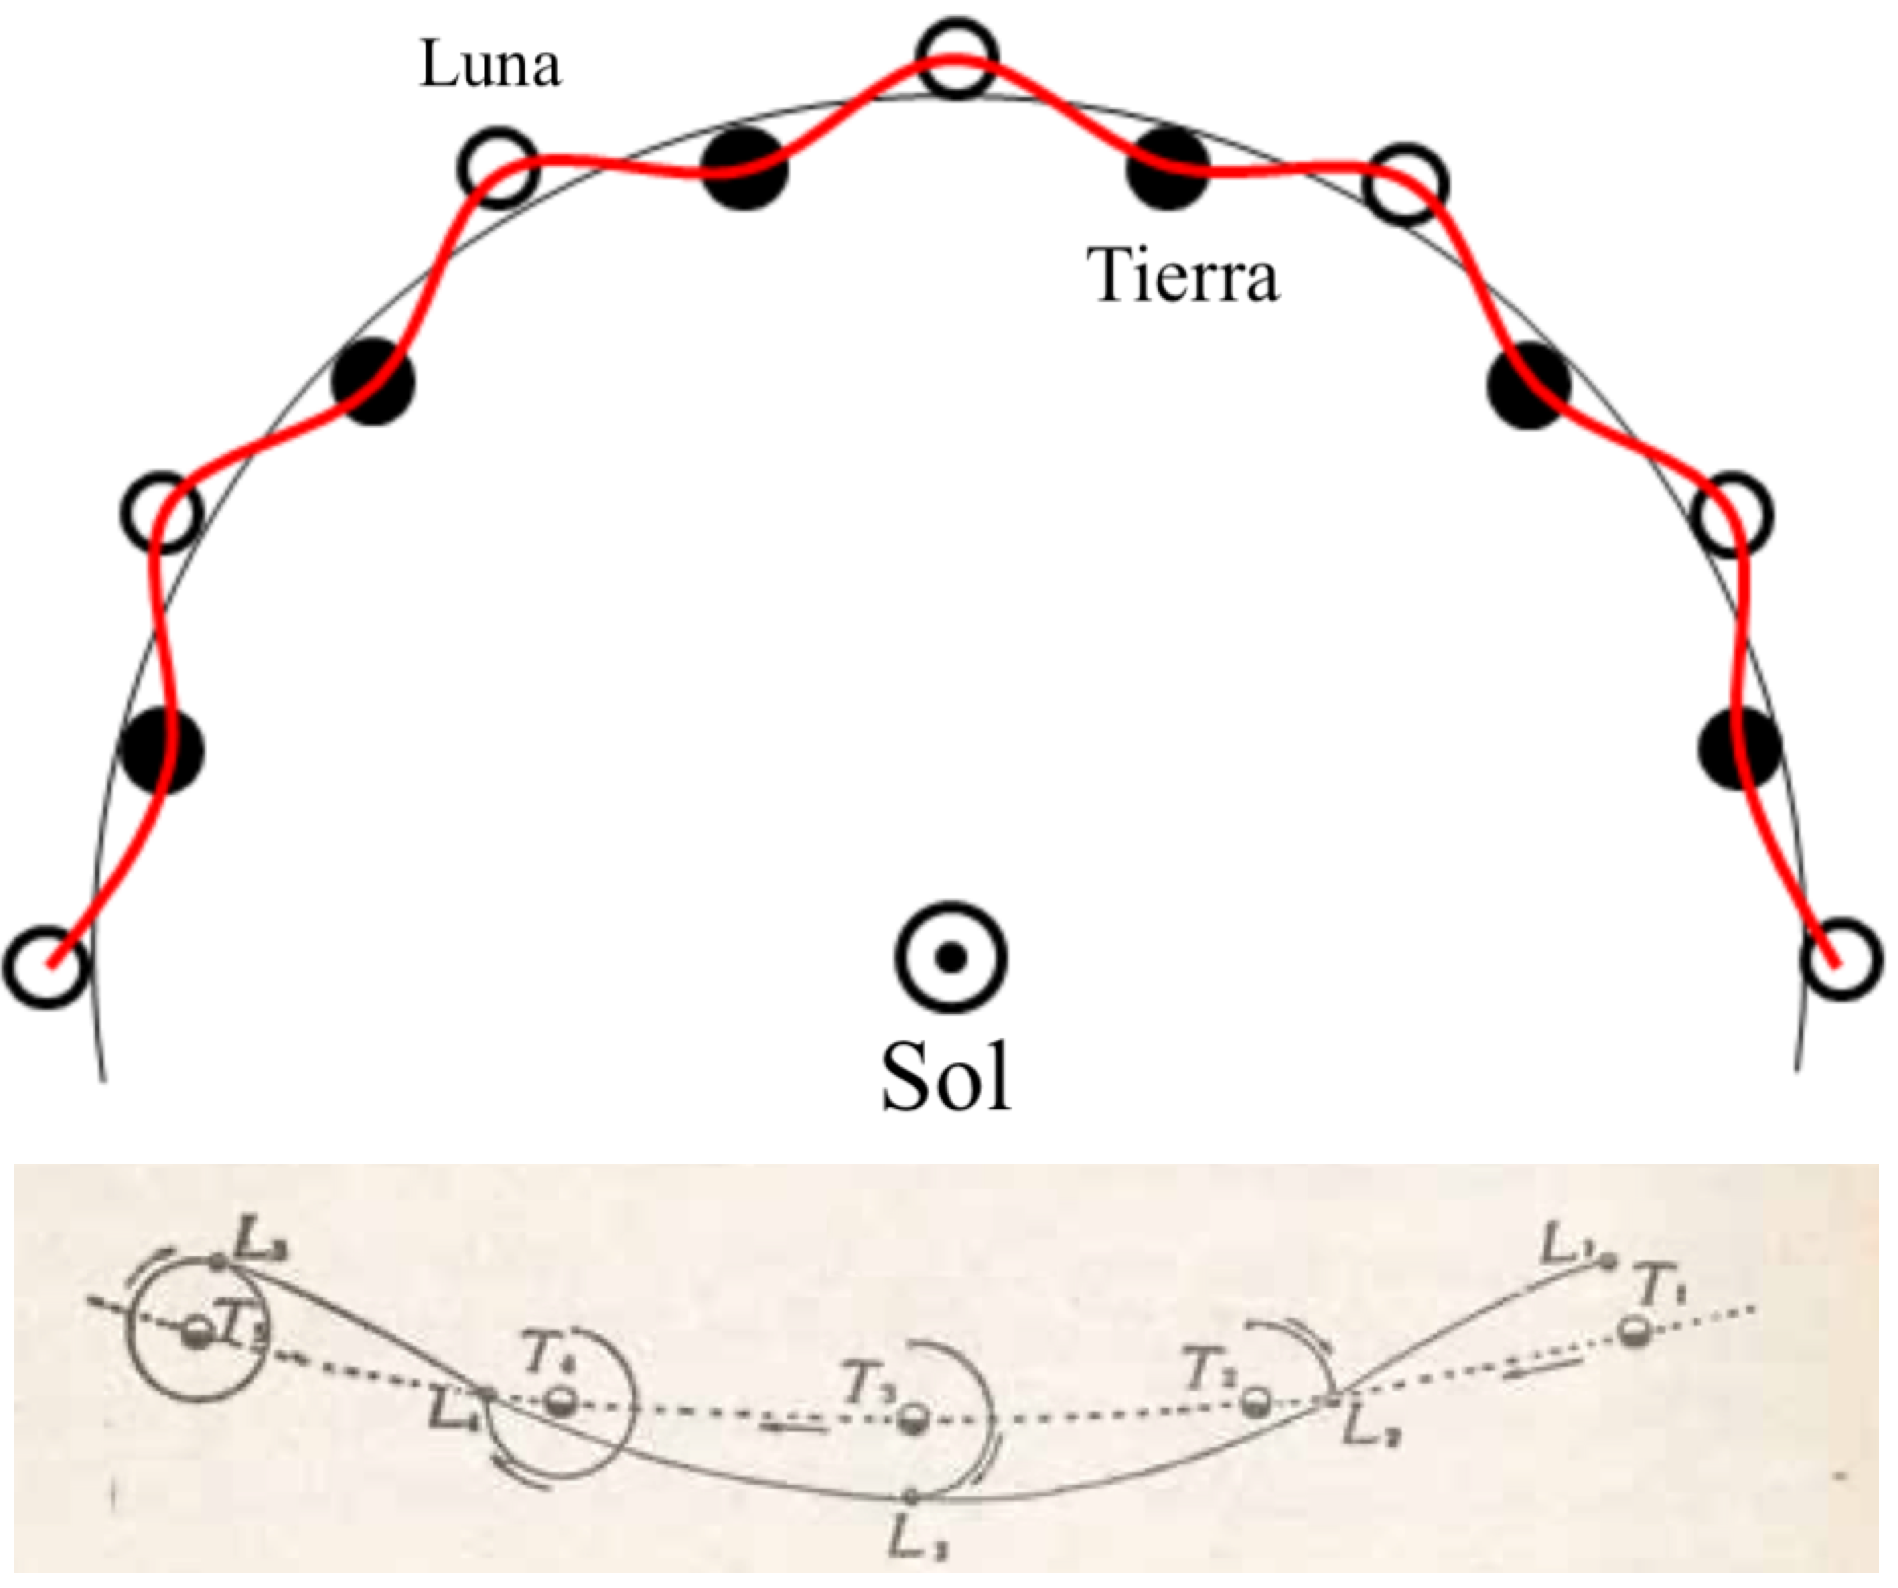
\includegraphics[width=.5\textwidth]{imagenes/imagenes02/T02IM01.png}
	\end{figure}
\end{multicols}

Un sistema de referencia es un conjunto de convenciones usado por un observador para poder medir la posición y otras magnitudes de un sistema físico. Las trayectorias medidas y el valor numérico de muchas magnitudes son relativas al sistema de referencia que se considere, por esa razón, se dice que el movimiento es relativo.

\begin{multicols}{2}
En mecánica clásica un sistema de referencia consta de un punto espacial fijo llamado origen $\mathcal O$, una base de vectores ortonormal orientada $\vec i,\; \vec j,\; \vec k$ \footnote{En el Apéndice \ref{Vectores} se recuerda el concepto de `Base OrtoNormal'.}  y un reloj para el origen de tiempos (dados dos sistemas de coordenadas de ese tipo, existe un giro y una traslación que relacionan las medidas de esos dos sistemas de coordenadas).
\begin{figure}[H]
		\centering
		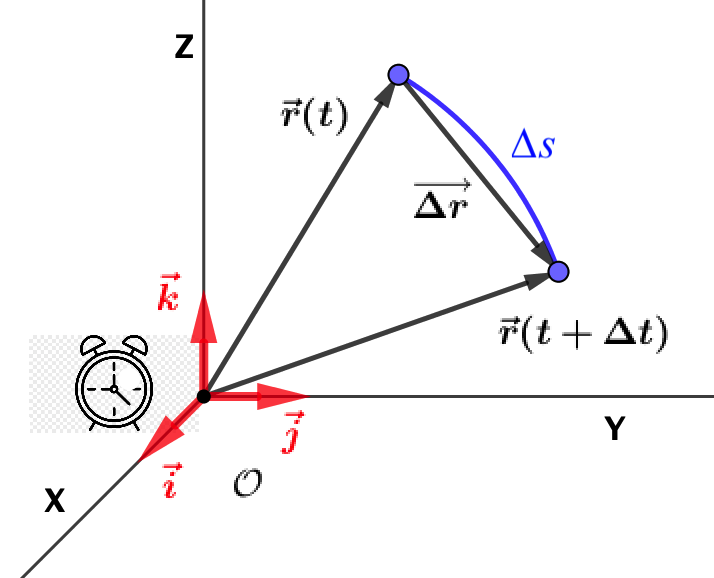
\includegraphics[width=.35\textwidth]{imagenes/imagenes02/T02IM02.png}
	\end{figure}
\end{multicols}

Cuando $\Delta t \to 0$, $\Delta \vec r$ es tangente a la trayectoria y $\abs{\Delta \vec r} \approx \Delta s$.

Por definición, la velocidad es:

\begin{equation}
\label{velocidad}
\subrayado{
 \vec v= \lim_{\Delta t\rightarrow 0 } \dfrac {\Delta \vec r}{\Delta t}	= \dv{\vec r}{t}
 }
\end{equation}


$\displaystyle \vec v= \lim_{\Delta t\rightarrow 0} \dfrac{\Delta \vec r}{\Delta s}\cdot \dfrac {\Delta s}{\Delta t} =\lim_{\Delta s\rightarrow 0} \dfrac{\Delta \vec r}{\Delta s}\cdot \lim_{\Delta t\rightarrow 0} \dfrac {\Delta s}{\Delta t}= \vec u_T \cdot v$

$\displaystyle \vec u_T=\lim_{t\rightarrow 0} \dfrac{\Delta \vec r}{\Delta s}$: dirección de la recta tangente a la trayectoria y módulo unidad.

$\displaystyle v=\lim_{t\rightarrow 0} \dfrac {\Delta s}{\Delta t}$: un escalar (número real).

\begin{equation}
\vec v=v\cdot \vec u_T
\end{equation}

El \colorbox{LightYellow}{vector velocidad} es, en todo momento, \colorbox{LightYellow}{tangente a la trayectoria} siendo $v$ su módulo (celeridad)\footnote{Celeridad = módulo del vector velocidad.}:
$\quad v=\abs{\vec v}=\sqrt{v_x^2+v_y^2+v_z^2}$

En el SI \emph{(Sistema Internacional de Unidades)}, la velocidad se mide en $\mathrm{m/s} = \mathrm{m\cdot s}^{-1}$

\section{Componentes cartesianas del vector velocidad}
Puesto que el vector de posición de la partícula que se mueve, $\vec r$, se puede expresar en coordenadas cartesinas en nuestro sistema de referencia como: $\;\;\vec r=x\cdot \vec i+y\cdot \vec j+z\cdot \vec k$, para el vector velocidad tendremos:

$\displaystyle \boldsymbol{\vec v}=\dv{\vec r}{t}= \dv{x}{t}\cdot \vec i+\dv{y}{t} \cdot \vec j+\dv{z}{t} \cdot \vec k  \boldsymbol{=v_x\cdot \vec i+v_y\cdot \vec j+v_z\cdot \vec k}$


\section{Movimiento de una partícula en un plano. Componentes polares de la velocidad} \label{velocidad-polares}

\begin{multicols}{2}
$\displaystyle \vec v= \dv{t} \vec 
r = \dv{t} (r\cdot \vec u_r)= $

$\displaystyle=\dv{r}{t} \cdot \vec u_r + r \cdot \dv{\vec u_r}{t}$

$\displaystyle  \dv{\vec u_r}{t}  \; \parallel \;\vec u_\theta$

Con $\quad \vec u_\theta \; \bot \; \vec u_r \quad (*)$ 
\begin{figure}[H]
		\centering
		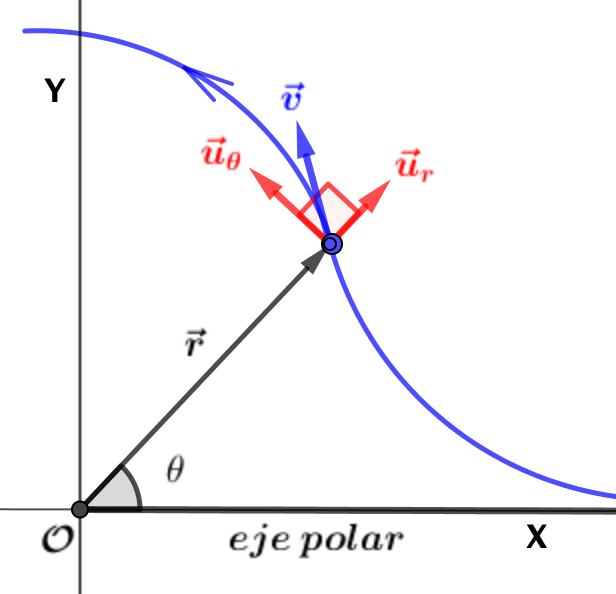
\includegraphics[width=.3\textwidth]{imagenes/imagenes02/T02IM03.png}
		\end{figure}
\end{multicols}

\begin{footnotesize}
\textcolor{gris}{$\displaystyle (*) \quad \dv{t} (\vec u_r \cdot \vec u_r)=\dv{t} 1=0$}

\textcolor{gris}{Por otra parte: $\displaystyle \dv{t} (\vec u_r \cdot \vec u_r)=\dv{\vec u_r}{t}\cdot \vec u_r+\vec u_r \cdot \dv{\vec u_r}{t}=2\vec u_r \dv{\vec u_r}{t}$}

\textcolor{gris}{Luego $\displaystyle \vec u_r \dv{\vec u_r}{t}=0 \Rightarrow \vec u_r \;\bot\; \dv{\vec u_r}{t}\;\ \parallel ;\vec u_\theta \qquad \Box$}

\textcolor{gris}{Hemos usado que $\vec u \cdot \vec v=\abs{\vec u} \;\abs{\vec v}\; \cos (\varphi_{\vec u, \vec v})$, por lo que $\vec u \cdot \vec v=0 \leftrightarrow \vec u \bot \vec v$ y que $\abs{\vec u_r}=\abs{\vec u_\theta}=1$. También que $\vec r=r\; \vec u_r$}
\end{footnotesize}

Transportando estos vectores al origen: \textcolor{gris}{$\alpha=90^o-\theta$}
\begin{multicols}{2}
$\begin{cases} \;\;\vec u_r=\;\;\cos \theta\; \vec i + \sin \theta\; \vec j \\ \\ \;\;\vec u_\theta = -\sin \theta \; \vec i + \cos \theta \;\vec j \end{cases}$
\begin{figure}[H]
		\centering
		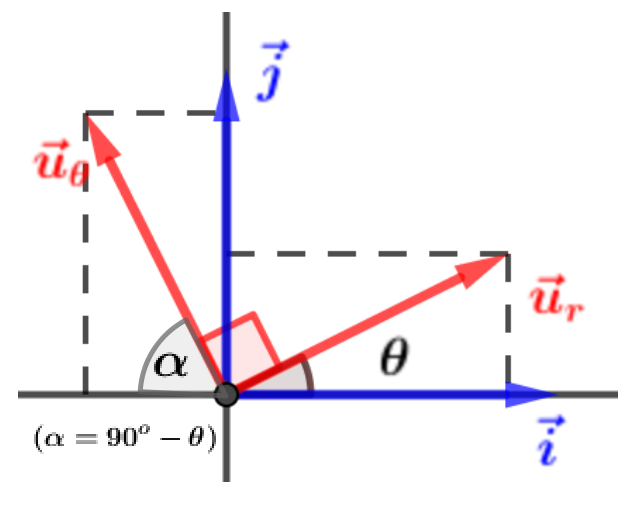
\includegraphics[width=.25\textwidth]{imagenes/imagenes02/T02IM04.png}
		\end{figure}
\end{multicols}

Derivando: $\quad \displaystyle \dv{\vec u_r}{t}=\dv{t} (\cos \theta\; \vec i + \sin \theta\; \vec j)=-\sin \theta \dv{\theta}{t} \; \vec i + \sin \theta \dv{\theta}{t} \; \vec j=(-sin \theta \;\vec i+ \cos \theta \; \vec j)\; \dv{\theta}{t} \quad \Rightarrow \qquad 	\boldsymbol{\dv{\vec u_r}{t}=\vec u_\theta \cdot \dv{\theta}{t}}\quad$ que es la relación matemática que buscábamos.

\begin{equation}
\label{veloc-polares}
\subrayado{
\vec v=\vec u_r \cdot \dv{r}{t} + \vec u_\theta \cdot r\cdot \dv{\theta}{t} 
}
\end{equation}

El primer de término es la `velocidad radial' y el segundo la `velocidad transversal'. Conclusión: \emph{La velocidad radial es perpendicular a la velocidad transversal}.

\section{Movimiento rectilíneo}

Movimiento rectilíneo es el que se realiza a lo largo de una línea recta. Llamamos eje $OX$ a la recta que describe esta trayectoria y fijamos un punto $\mathcal O$ como origen. La posición del objeto al cabo de de un tiempo $T$ viene dada por el escalar, en este caso, $r(t)$ que mide la distancia del móvil al origen $\mathcal O$. En estas condiciones:

$\displaystyle \vec v= \dv{\vec r}{t} \to \int_{r_0}^{r} \dd r=\int_{t_0}^{t}v\; \dd t \quad \Rightarrow \qquad  \quad r-r_0=\int_{t_0}^{t}v\; \dd t $

En el caso particular de que $ \; v=cte	\;$, independiente del tiempo, la expresión anterior queda como: $ \;\; r-r_0=v\; ( t-t_0 ) $

Consideremos ahora que el observador no está situado sobre la recta de la trayectoria o eje de movimiento:


\begin{multicols}{2}
$\displaystyle \vec v=\dv {\vec r}{t}\to \int_{\vec r_0}^{\vec r} \dd r = \int_{t_0}^{t} \vec v \ \dd t$ 

de donde: $\vec r-\vec r_0=\displaystyle \int_{t_0}^{t} \vec v \ \dd t$

\begin{figure}[H]
		\centering
		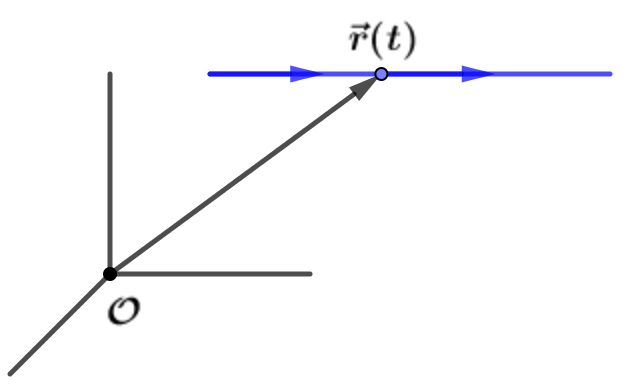
\includegraphics[width=.25\textwidth]{imagenes/imagenes02/T02IM05.png}
		\end{figure}
\end{multicols}
En el caso particular de que $\boldsymbol{ \;\vec v= \overrightarrow{cte}\; }$, se tiene:

\begin{equation}
\label{MRU}
	 \vec r-\vec r_0=\vec v\; (t-t_0) 
\end{equation}

que es la ecuación del \textbf{MRU} (movimiento rectilíneo uniforme, $\vec v = \overrightarrow{cte}$) en tres dimensiones.

\vspace{-4mm}\section{Movimiento circular. Velocidad angular.}

Llamamos movimiento circular a aquel que describe una circunferencia, por tanto, tiene lugar en un plano. Usaremos coordenadas polares que son más útiles en este caso.

Al ser la trayectoria una circunferencia, $R=\abs{\vec R}=cte$, por lo que:

\begin{multicols}{2}

$\displaystyle \vec v=\dv{\vec R}{t}=\dv{(R\;\vec u_R)}{t}=$

$\displaystyle =\cancelto{0}{\dv{R}{t}}\;\vec u_R+R\; \dv{\vec u_R}{t}$
\begin{figure}[H]
		\centering
		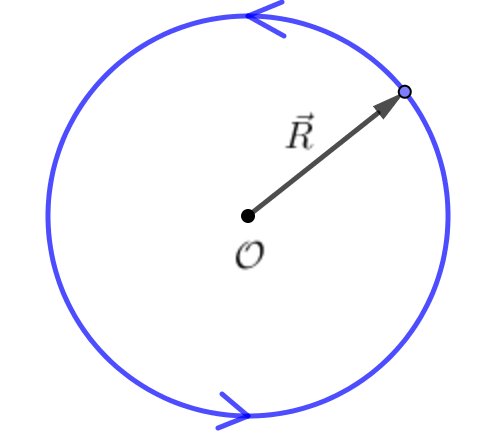
\includegraphics[width=.2\textwidth]{imagenes/imagenes02/T02IM06.png}
		\end{figure}
\end{multicols}

Recordando la ecuación \ref{veloc-polares}:
$\qquad \displaystyle \vec v=R\cdot \dv{\theta}{t}\;\vec u_\theta=R\cdot \omega \; \vec u_\theta$,

Siendo $\displaystyle \omega=\dv{\theta}{t}$ el módulo de la velocidad angular (ángulo barrido en la unidad de tiempo), que en el $SI\;$\footnote{ SI= Sistema Internacional de unidades.} se mide en $\mathrm{s}^{-1}$. Es usual expresarla en $\text{rad}\cdot \mathrm{s}^{-1}$ o $\text{rpm}$.\footnote{ rpm=revoluciones por minuto.}

Supongamos ahora que el observador no se encuentra situado en el centro de la circunferencia que describe la partícula que se mueve sino en una recta perpendicular a ella que pasa por su centro.

\begin{multicols}{2}
Respecto de $\mathcal O'$

$\displaystyle \vec v = \textcolor{gris}{\vec v_{\mathcal O'}}=\dv{\overrightarrow{ r }}{t} = \dv{t}(\overrightarrow{\mathcal O \mathcal O'}+\vec R )=$

$\displaystyle =\dv {\vec R} {t}=R\cdot \omega\; \vec u_\theta\; ; \qquad \textcolor{gris}{\overrightarrow{\mathcal O \mathcal O'}=\overrightarrow{cte}}$

\begin{figure}[H]
		\centering
		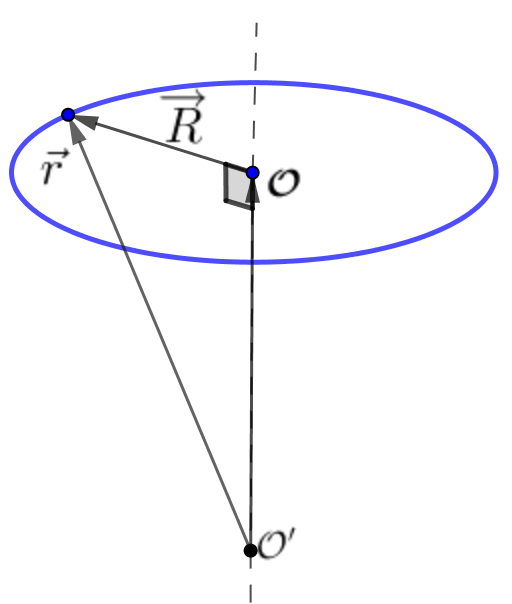
\includegraphics[width=.20\textwidth]{imagenes/imagenes02/T02IM07.png}
		\end{figure}
\end{multicols}

\begin{multicols}{2}
Sea $\mathcal O'$ un punto cualquiera de la recta perpendicular a la trayectoria que pasa por el centro, $(\mathcal O)$, de la figura:
$\quad R=r\cdot \sin \alpha$

Luego $\quad \vec v= \omega \cdot r \cdot \sin \alpha \;\; \vec u_\theta$

Recordando la definición de `producto vectorial' de dos vectores (y la regla del sacacorchos para determinar su sentido),

\begin{figure}[H]
		\centering
		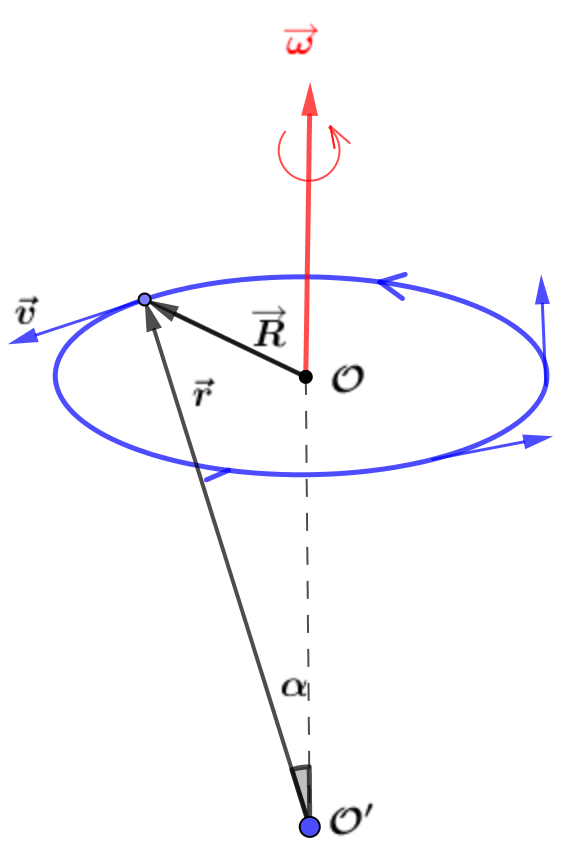
\includegraphics[width=.25\textwidth]{imagenes/imagenes02/T02IM08.png}
		\end{figure}
\end{multicols}

\begin{equation}
\label{v-angular}
\subrayado{
\vec v=\vec \omega \times \vec r
}
\end{equation}
donde $\vec \omega$ es el vector velocidad angular.

El vector velocidad angular es perpendicular al plano del movimiento en es sentido de avance de un sacacorchos que gira en el mismo sentido en que lo hace la partícula, en módulo se tiene que $ v=\omega\; r\; \sin \alpha$. 

\begin{multicols}{2}
$\quad$

\emph{Nótese que esto solo es válido para movimientos circulares con el observador situado perpendicularmente al centro de la treyectoria, es decir, siempre que $R=cte \; \wedge \; alpha=cte$.}  
\begin{figure}[H]
		\centering
		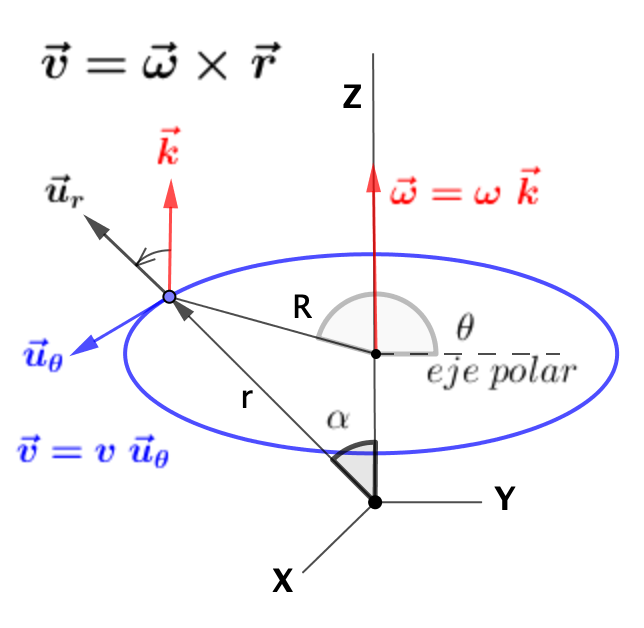
\includegraphics[width=.4\textwidth]{imagenes/imagenes02/T02IM09.png}
		\end{figure}
\end{multicols}

Como $\displaystyle \omega=\dv{\theta}{t}\to  \int_{\theta_0}^{\theta}\dd \theta = \int_{t_0}^t \omega \;\dd t \Rightarrow \;\; \;\theta-\theta_0=\int_{t_0}^t \omega \;\dd t\;$

En el caso particular en que $\; \theta = cte$, tendremos: $\;\theta-\theta_0= \omega \;(t-t_0)\;$

Un movimiento es \textbf{periódico} si al pasar un determinado tiempo $\boldsymbol{T}$ llamado \textit{\textbf{periodo}},  todas las variables que describen el movimiento vuelven a tomar el mismo valor. \textit{El movimiento circular uniforme, en que $\omega=cte$, es periódico.}

\textbf{Relación entre $\boldsymbol{T}$ y $\boldsymbol{\omega}$}


\begin{multicols}{2}
Empezamos a contar el tiempo (\emph{origen de tiempos}) cuando la partícula está en el punto A en que el ángulo, medido desde el eje polar, es $\theta_0$. Las variables que describan el movimiento volverán a tomar el mismo valor al cabo de una vuelta:

\begin{figure}[H]
		\centering
		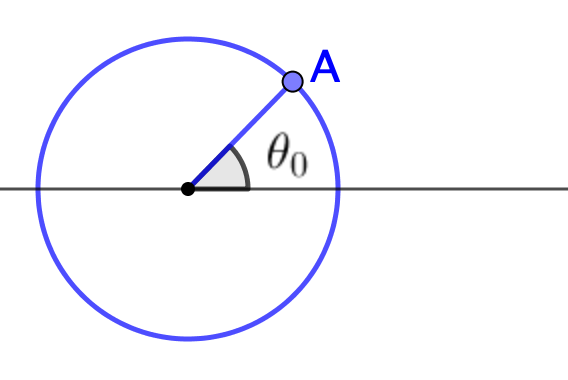
\includegraphics[width=.45\textwidth]{imagenes/imagenes02/T02IM10.png}
		\end{figure}
\end{multicols}

$\theta=\theta_0+\omega \; T \to $, al cabo de una vuelta $\theta=\cancel{\theta_0}+2\pi=\cancel{\theta_0}+\omega \; T \to 2\pi=\omega \; T$

de donde:

\begin{equation}
\label{periodo-vel-angular}
T = \dfrac {2\pi}{\omega} \qquad \vee \qquad \subrayado{\omega=\dfrac{2\pi}{T}}	
\end{equation}

$T$ en $s$. Se llama \textbf{\emph{frecuencia, $\nu$}} a la inversa del periodo y se expresa en $s^{-1}\;(=Hz=rps)$\footnote{rps: revoluciones por segundo}.

\begin{equation}
T=\dfrac 1 \nu	 \qquad \qquad \omega=2\pi\; \nu
\end{equation}

La velocidad angular se usa para movimientos angulares (para movimientos aproximadamente circulares se usa la velocidad angular media).

\section{Aceleración}

La \emph{aceleración} es una magnitud vectorial íntimamente ligada con la \emph{fuerza}. Por definición, la aceleración es: 

\begin{multicols}{2}

\begin{figure}[H]
		\centering
		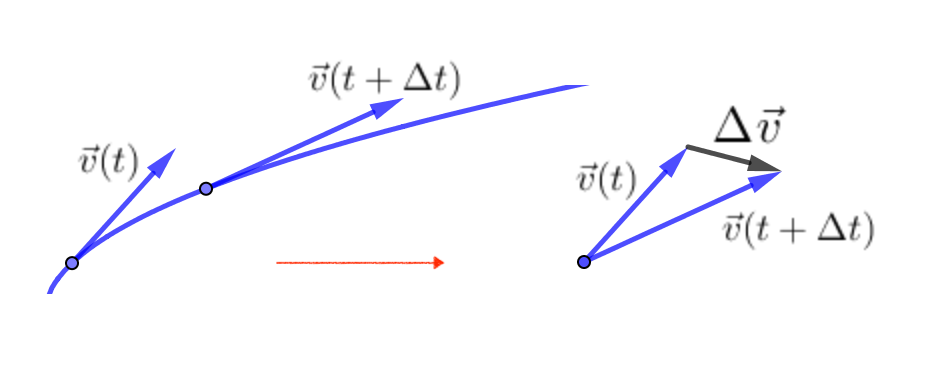
\includegraphics[width=.6\textwidth]{imagenes/imagenes02/T02IM11.png}
		\end{figure}
\vspace{3mm}
\begin{equation}
\label{aceleracion}
\subrayado{
\vec a= \lim_{\Delta t\rightarrow 0 } \dfrac{\Delta \vec v}{\Delta t}=\dv{\vec v}{t}	
}
\end{equation}
\end{multicols}

\begin{multicols}{2}
Características de $\vec a$:

$\quad$

Mira siempre hacia el interior de la concavidad de la trayectoria.
\begin{figure}[H]
		\centering
		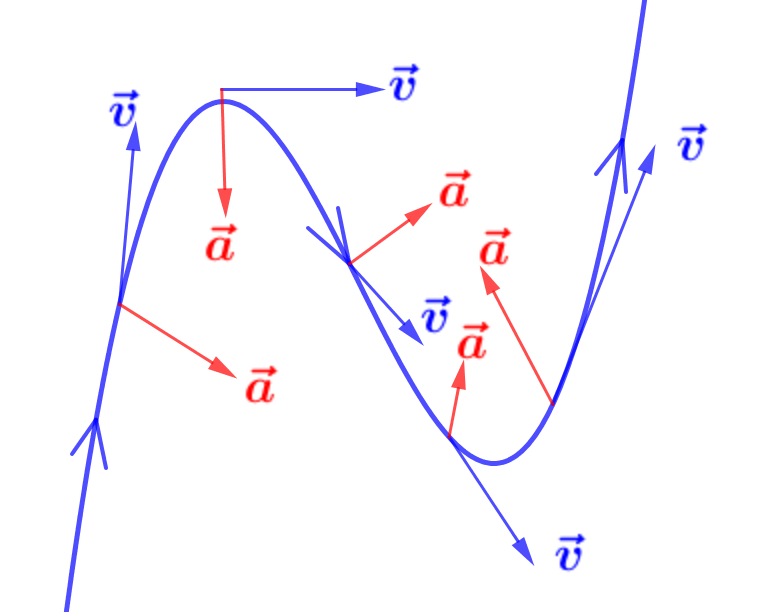
\includegraphics[width=.3\textwidth]{imagenes/imagenes02/T02IM12.png}
		\end{figure}
\end{multicols}

\begin{figure}[H]
		\centering
		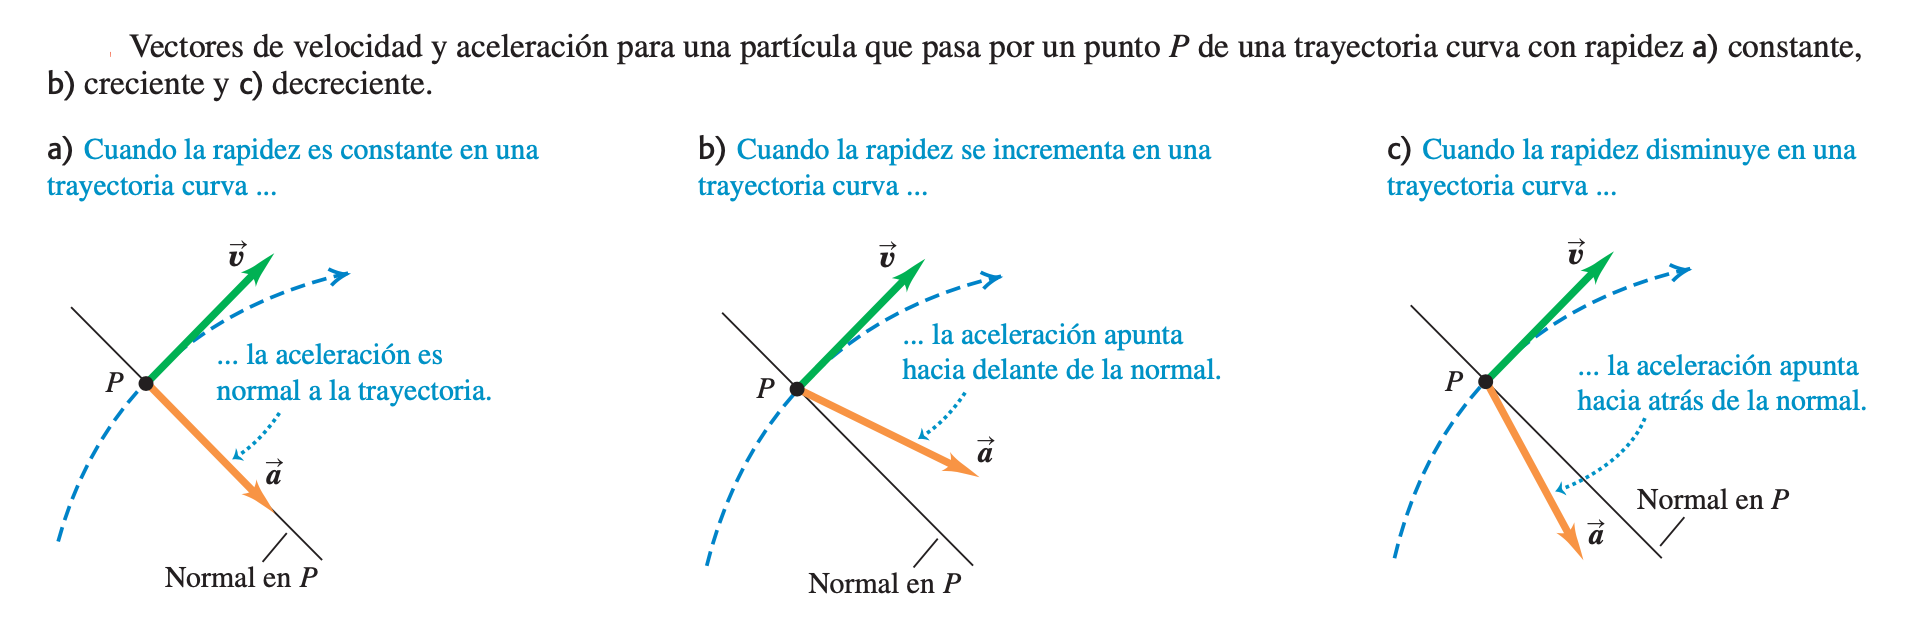
\includegraphics[width=1\textwidth]{imagenes/imagenes02/T02IM15.png}
		\end{figure}

Resolvamos el problema de determinar $\vec v$ y $\vec r$ conocido el vector $\vec a$ y las condiciones iniciales $\vec v_0$ y $\vec r_0$:

De la definición de aceleración, ecuación \ref{aceleracion}: $\;\;\dd \vec v= \vec a\; \dd t\;$ . Integrando entre $t_o$ y $t$, intervalo en que las velocidades son $\vec v_0$ y $\vec v$ respectivamente:

$\displaystyle \int_{\vec v_0}^{\vec v}\dd \vec v= \int_{t_0}^{t} \vec a\; \dd t \quad \to \qquad \vec v=\vec v_0+\int_{t_0}^{t} \vec a\; \dd t$

\subsection{Movimiento rectilíneo uniformemente acelerado}

Particularizemos para el caso en que $\boldsymbol{ \vec a=\overrightarrow{cte} }$, \textbf{MRUA} \emph{(Movimiento rectilíneo uniformemente acelerado --$\vec a=\overrightarrow{cte}$--):}

En estas condiciones, $\vec a=\overrightarrow{cte}$, se tiene que:

\begin{equation}
\label{MRUAv}
	\vec v=\vec v_0+\vec a\; (t-t_0)
\end{equation}

$\displaystyle \vec v=\dv{\vec r}{t} \to \dd \vec r=\vec v\dd t : \quad \int_{\vec r_0}^{\vec r}\dd \vec r=\int_{t_0}^t \vec v\;\dd t \to$, teniendo en cuenta \ref{MRUAv}:

$\displaystyle \vec r-\vec r_0=\int_{t_0}^t 
\qty(\; \vec v_0+\vec a\; (t-t_0) \;)
\; \dd t;\; \qquad \vec a=\overrightarrow{cte} \; \wedge \; \vec v_0=\overrightarrow{cte'} \Rightarrow\;:$

\begin{equation}
\label{MRUAr}
	\vec r=\vec r_0+ \vec v_0\; (t-t_0)+\dfrac 1 2 \vec a\; (t-t_0)^2
\end{equation}

Las ecuaciones del MURA en una dimensión (observador situado en la recta de la trayectoria) las ecuaciones son:
$$v=v_0+a\;(t-t_o) \qquad \wedge \qquad r=r_0+v_0\;(t-t_0)+\dfrac 1 2 \; a \; (t-t_0)^2$$

\emph{Cuando la aceleración es constante, la trayectoria es una parábola} ($r \propto t^2$).


\subsection{Componentes cartesianas de la aceleración}

$\displaystyle \vec a=\dv{\vec v}{t}=\textcolor{gris}{
\dv{t}\left( \dv{\vec r}{t}  \right)
}=\dv[2]{\vec r}{t}$

$\displaystyle 
\vec a=\dv{v_x}{t}\;\vec i+\dv{v_y}{t}\;\vec j+\dv{v_z}{t}\;\vec k
\qquad \qquad
\vec a= \dv[2]{x}{t}\;\vec i+\dv[2]{y}{t}\;\vec j+\dv[2]{z}{t}\;\vec k$

$\displaystyle \vec a=a_x\;\vec i+a_y\;\vec j+a_z\;\vec k \quad \qquad \to \qquad \abs{\vec a}=\sqrt{a_x^2+a_y^2+a_z^2}$

 \subsection{Movimiento en un plano.  Aceleración en coordenadas polares}

$\displaystyle \vec a=\dv{\vec v}{t}\;,\qquad$
por \ref{veloc-polares}: $\quad \vec v=\vec u_r \cdot \dv{r}{t} + \vec u_\theta \cdot r\cdot \dv{\theta}{t} $

$\begin{cases} \;\;\vec u_r=\;\;\cos \theta\; \vec i + \sin \theta\; \vec j \\  \;\;\vec u_\theta = -\sin \theta \; \vec i + \cos \theta \;\vec j \end{cases}  \hspace{-3mm} \to \;\;
\displaystyle \dv{\vec u_r}{t}=\vec u_\theta\; \dv{\theta}{t}\;;  \qquad 
\displaystyle \dv{\vec u_\theta}{t}=-\vec u_r \dv{\theta}{t}\; (*)$




$\displaystyle \vec a =\dv{\vec u_r}{t}\; \dv{r}{t} 
+ \vec u_r\; \dv[2]{r}{t} 
+ \dv{\vec u_\theta}{t}\;r\;\dv{\theta}{t}
+\vec u_\theta\;\dv{r}{t}\;\dv{\theta}{t}
+\vec u_\theta\;r\;\dv[2]{\theta}{t}= \quad (\overleftarrow{*}) \; \Rightarrow$

\begin{equation}
\label{aceleracionpolares}	
\displaystyle \vec a\;=\;\vec u_r\;\left[ \dv[2]{r}{t}-r\left(\dv{\theta}{t} \right)^2 \right] + \vec u_\theta \; \left[ 2\;\dv{r}{t}\;\dv{\theta}{t}+r\;\dv[2]{\theta}{t} \right]
\end{equation}

Estas son las componentes polares del vector aceleración y son muy útiles para trabajar en el plano. El primer término es la `componente radial' de la aceleración (responde de la aceleración de la aceleración). El segundo término es la `componente transversal' de la aceleración. Ambos términos son perpendiculares ($\;\vec u_r\;\bot\;\vec u_\theta$). 

\subsection{Componentes intrínsecas de la aceleración}

Supongamos que una partícula $P$ describe la trayectoria que aparece el la siguiente figura. La dirección normal es perpendicular a la tangente y en estas direcciones representamos las componentes normal y tangencial del vector aceleración. A estas componentes, $\vec a_T$ y $\vec a_N$ se les llama \emph{componentes intrínsecas de la aceleración.}

\begin{multicols}{2}
$\displaystyle \vec a=\dv{\vec v}{t}=\dv{t}(v\cdot \vec u_T)=$

$\displaystyle =\vec u_T\; \dv{v}{t}+v\;\dv{\vec u_T}{t}$

$\begin{cases} \;\;\vec u_T=\;\;\cos \theta\; \vec i + \sin \theta\; \vec j \\  \;\;\vec u_N = -\sin \theta \; \vec i + \cos \theta \;\vec j \end{cases} \cdots \to $

$\displaystyle \dv{\vec u_T}{t}=\vec u_N\; \dv{\theta}{t}\;;  \;\; 
\displaystyle \dv{\vec u_N}{t}=-\vec u_T \dv{\theta}{t}$

\begin{figure}[H]
		\centering
		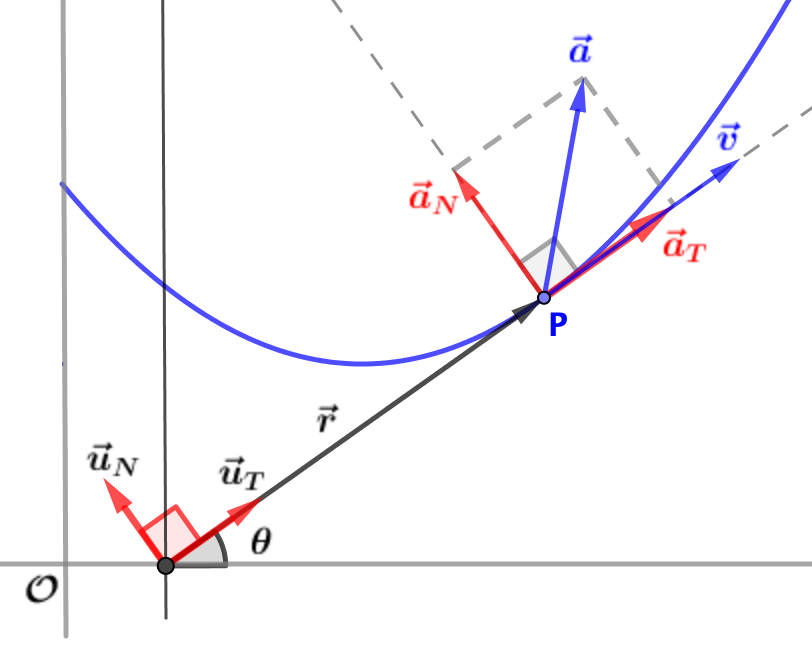
\includegraphics[width=.4\textwidth]{imagenes/imagenes02/T02IM13.png}
		\end{figure}
\end{multicols}


Al pasar de $\;t\;$ a $\;t+dt\;$, el ángulo polar cambia $\;\dd \theta=\theta(t+dt)-\theta(t)$.

Por otro lado, de la relación \emph{arco=ángulo por radio} (cuando el ángulo se expresa en radianes) tenemos:

$\dd s=\dd \theta \cdot \rho\;$ Donde $\rho$ es el llamado \emph{radio de curvatura}.

Como $\; \displaystyle \dv{\theta}{t}=\dv{\theta}{s}\cdot \dv{s}{t}=\dfrac 1 \rho \; v$ 

\begin{figure}[H]
		\centering
		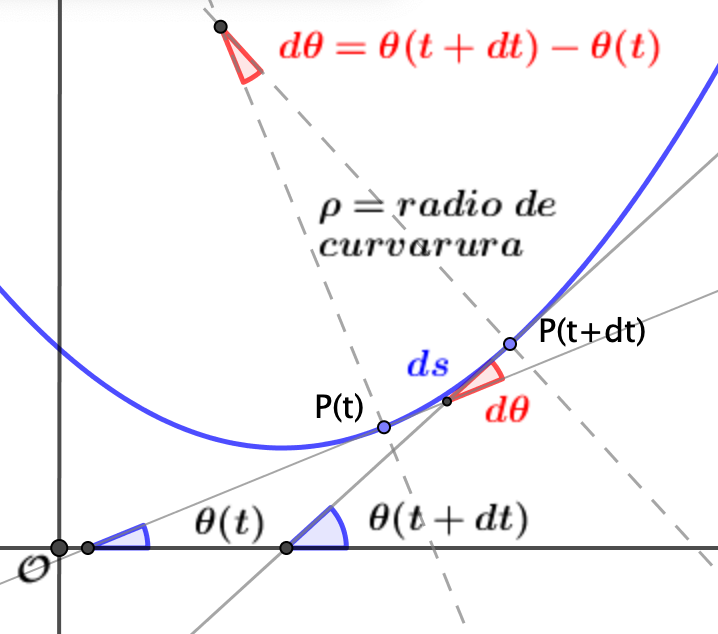
\includegraphics[width=.5\textwidth]{imagenes/imagenes02/T02IM14.png}
		\end{figure}


Se tiene que:

\begin{equation}
\subrayado{
\label{intrinsecas}
\vec a\;=\;\vec u_T\; \dv{v}{t} \;+\; \vec u_N	\; \dfrac {v^2}{\rho}
}
\end{equation}

\begin{miparrafo}

\noindent \textbf{---} La aceleración tangencial, $a_T$, mide el cambio del módulo del vector velocidad (si la partícula viaja más deprisa o más despacio) y es tangente, en todo momento, a la trayectoria.

\vspace{3mm}
\noindent \textbf{---}  La aceleración normal, $a_N$, mide el cambio de la dirección del vector velocidad y es perpendicular (normal) a la trayectoria en todo momento.

\end{miparrafo}

En coordenadas polares, el módulo del vector aceleración se mide por:
$$\displaystyle \abs{\vec a}=\sqrt{\left(\dv{v}{t} \right)^2+\dfrac {v^4}{\rho^2}}$$

-- Para MR, aquellos en los que que no cambia la dirección del vector velocidad, $a_n=0 \to \; \rho = \infty $ (recta).

-- Pra MRU, $\vec v=\overrightarrow{cte}$, tenemos $\abs{\vec v}=cte \to \displaystyle \dv{v}{t}=0 \to a_T=0$

OJO: $\displaystyle \dv{v}{t}= \dv{\abs{\vec v}}{t} \; \neq \; \abs{\dv{\vec v}{t}}$.

\begin{figure}[H]
		\centering
		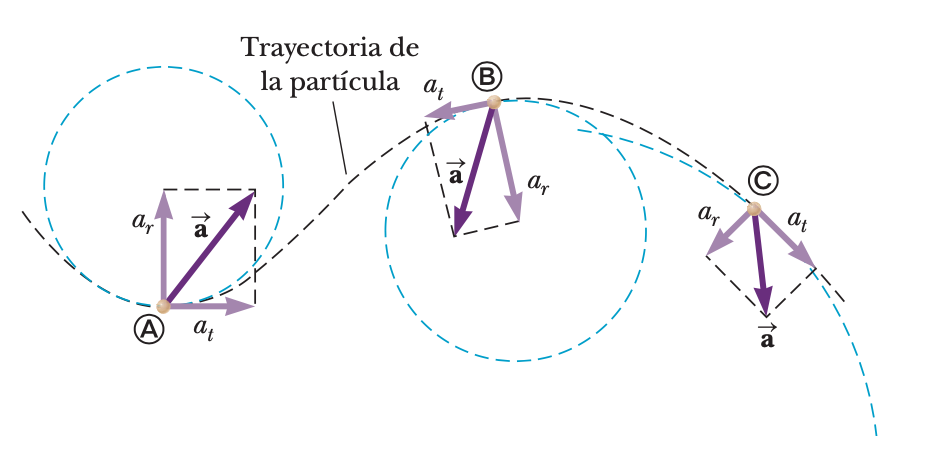
\includegraphics[width=.8\textwidth]{imagenes/imagenes02/T02IM39.png}
		\end{figure}
\vspace{-10mm} %************
\rule{150pt}{0.4pt}

\begin{multicols}{2}
ATENCIÓN: 

No confundir las componentes polares de la aceleración, en las direcciones $\vec u_r$ y $\vec u_\theta$ con las componentes intrínsecas, en las direcciones tangencial $\vec u_T$ y normal $\vec u_n$.
\begin{figure}[H]
		\centering
		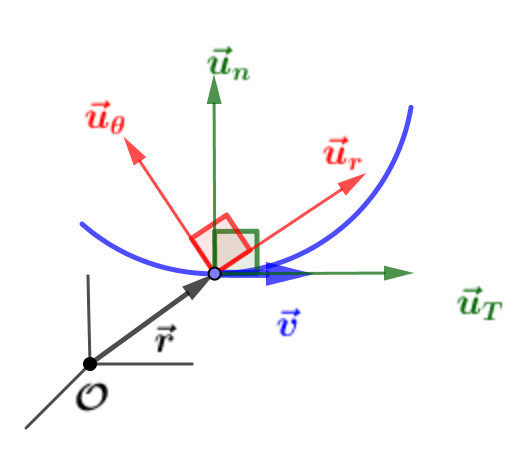
\includegraphics[width=.4\textwidth]{imagenes/imagenes02/T02IM35.png}
		\end{figure}
\end{multicols}
\vspace{-10mm} %**************************************
\rule{150pt}{0.4pt}

\textbf{Los movimientos se pueden clasificar según las componentes intrínsecas de su aceleración. }
\vspace{-2mm}\begin{enumerate}
\vspace{-2mm}\item $a_T=0$ 
	\vspace{-2mm}\begin{enumerate}
	\vspace{-2mm}\item $a_N=0$. Movimiento rectilíneo a velocidad constante. 
	\vspace{-2mm}\item $a_N=cte$. Movimiento circular uniforme. 
	\vspace{-2mm}\item $a_N\neq cte$. Movimiento circular acelerado. 
	\vspace{-2mm}\end{enumerate}
\vspace{-2mm}\item $a_N=0$ 
	\vspace{-2mm}\begin{enumerate}
	\vspace{-2mm}\item $a_T=0$.   Movimiento rectilíneo a velocidad constante. 
	\vspace{-2mm}\item $a_T=cte$. Movimiento rectilíneo uniformemente acelerado. 
	\vspace{-2mm}\item $a_T\neq cte$. Movimiento rectilíneo acelerado. 
	\end{enumerate}
\vspace{-2mm}\item  $a_N=0;\; a_T=0$.  Movimiento curvilíneo.
\end{enumerate}

\vspace{10mm} %***********************************
\begin{figure}[H]
		\centering
		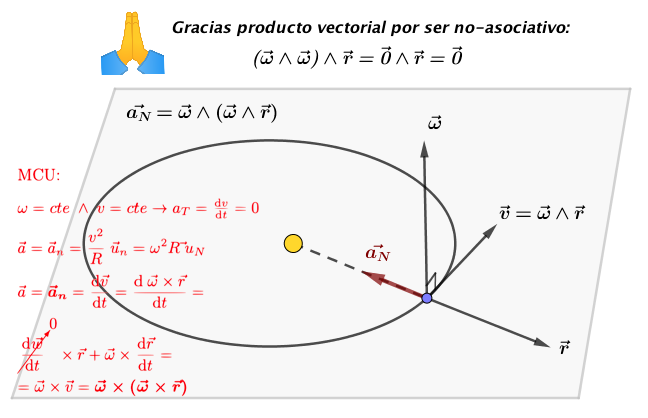
\includegraphics[width=.9\textwidth]{imagenes/imagenes02/T02IM34.png}
		\end{figure}

\newpage %**********************
	\begin{figure}[H]
		\centering
		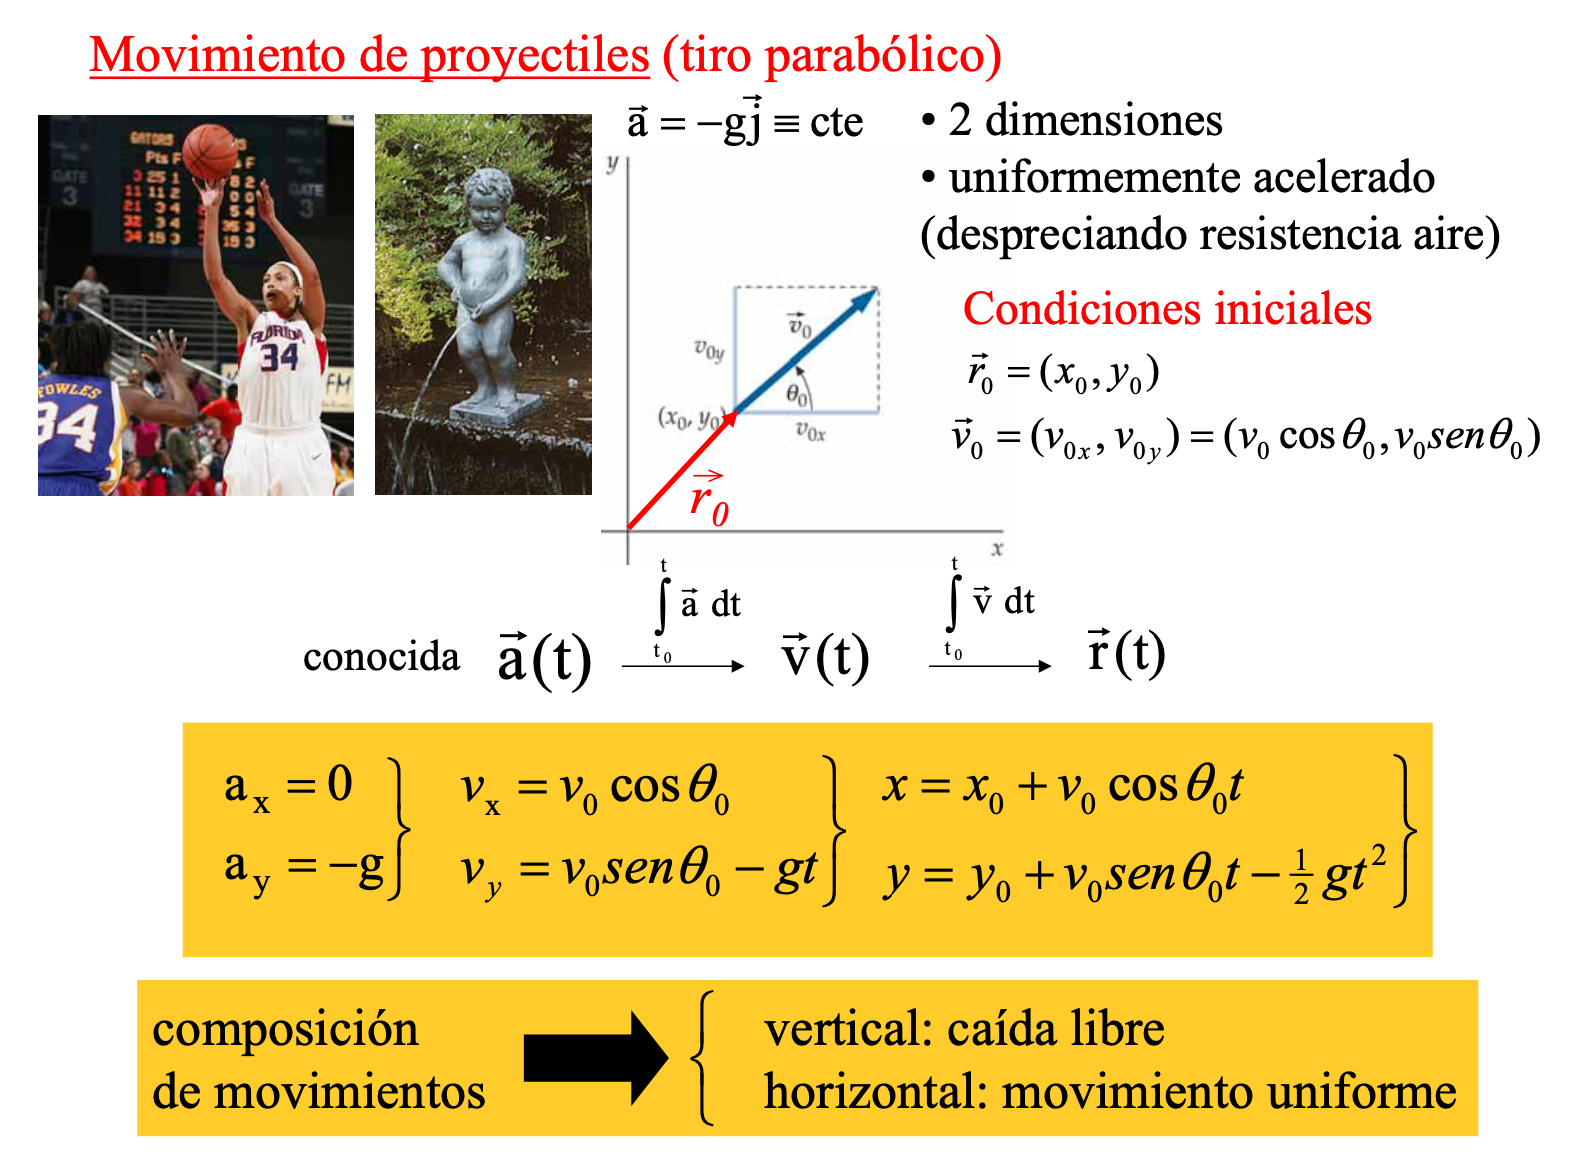
\includegraphics[width=.95\textwidth]{imagenes/imagenes02/T02IM22.png}
		\end{figure}		
	\begin{figure}[H]
		\centering
		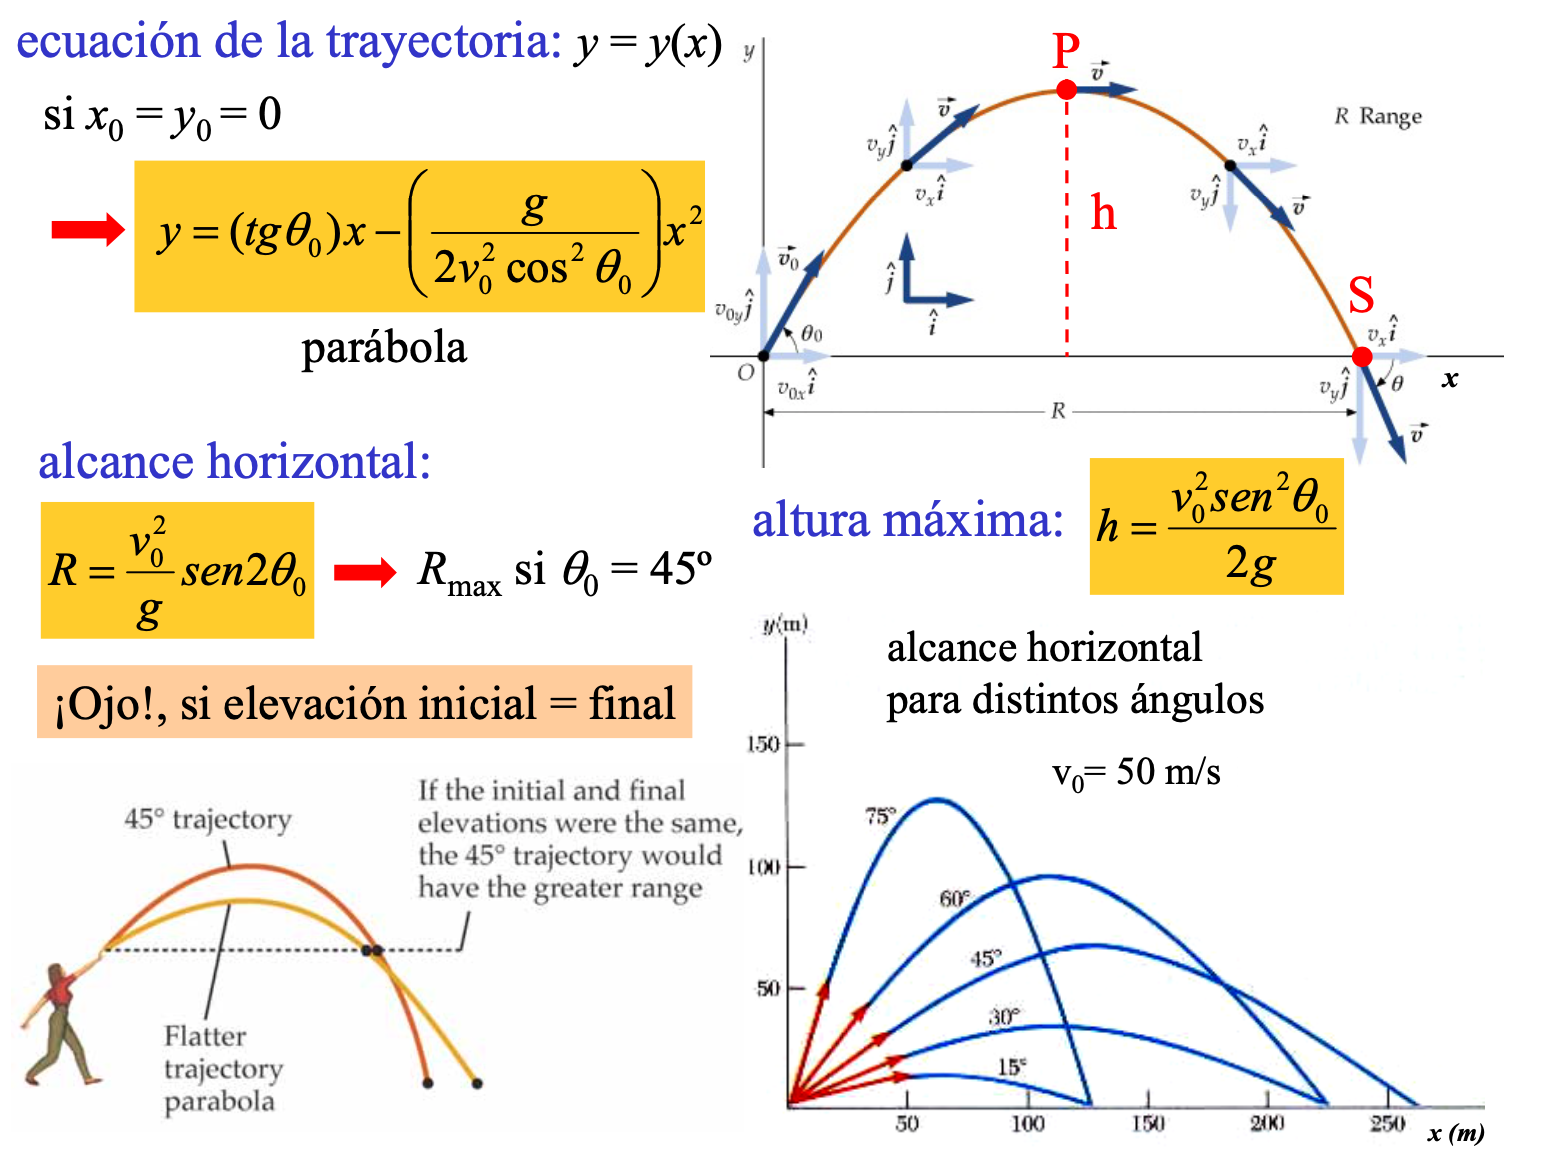
\includegraphics[width=.95\textwidth]{imagenes/imagenes02/T02IM23.png}
		\end{figure}
	\begin{figure}[H]
		\centering
		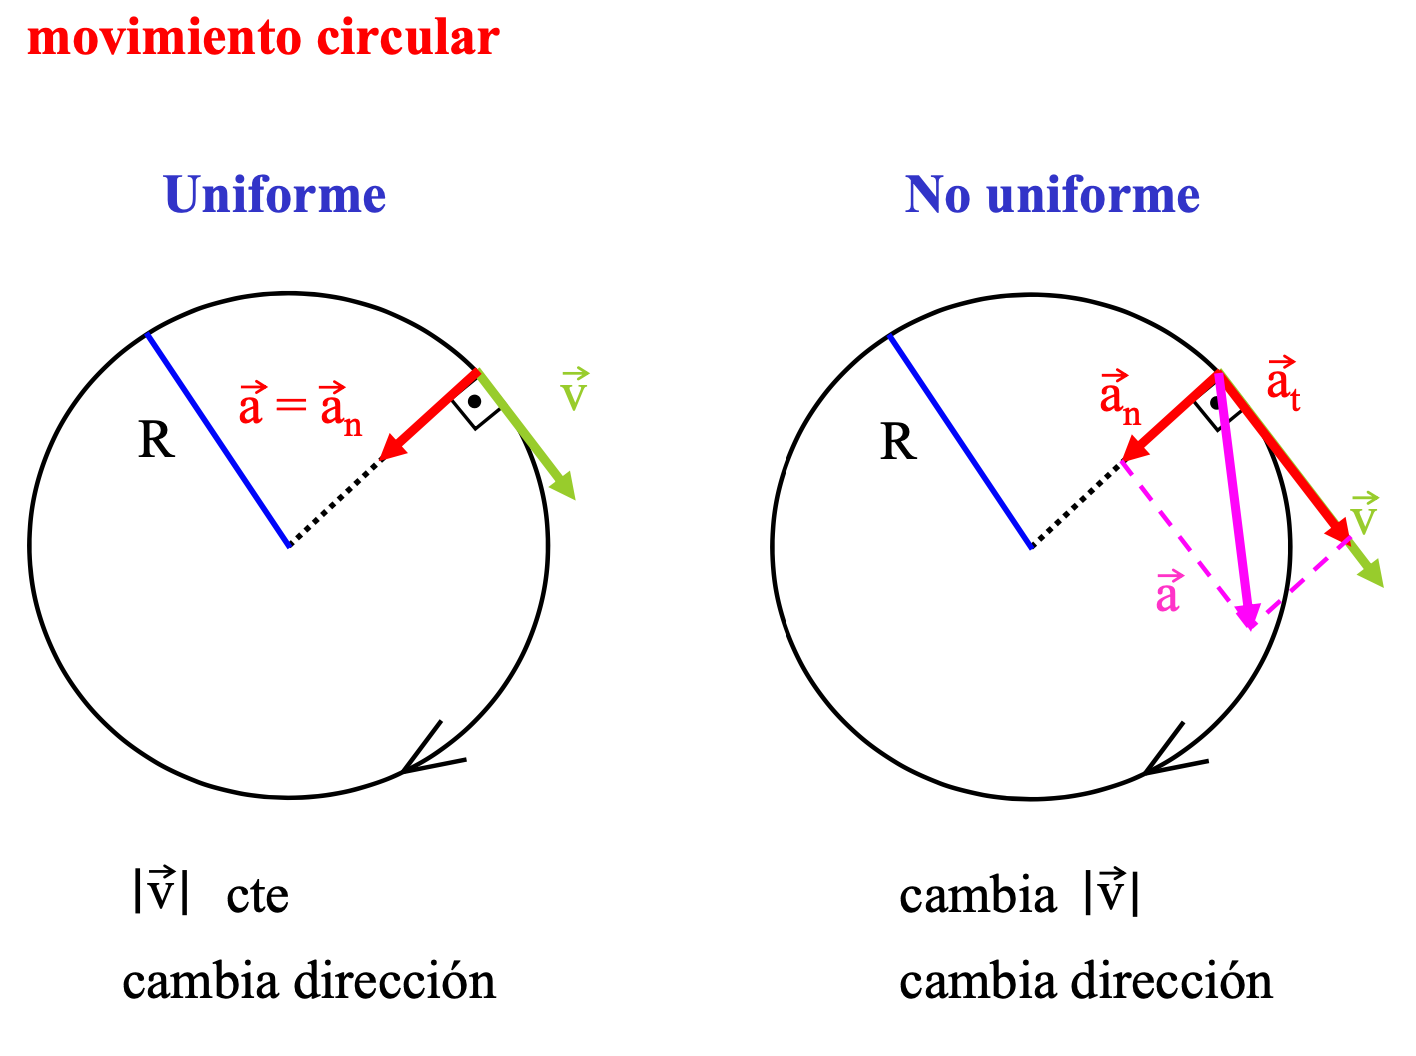
\includegraphics[width=.6\textwidth]{imagenes/imagenes02/T02IM29.png}
		\end{figure}
	\vspace{-4mm}\begin{figure}[H]
		\centering
		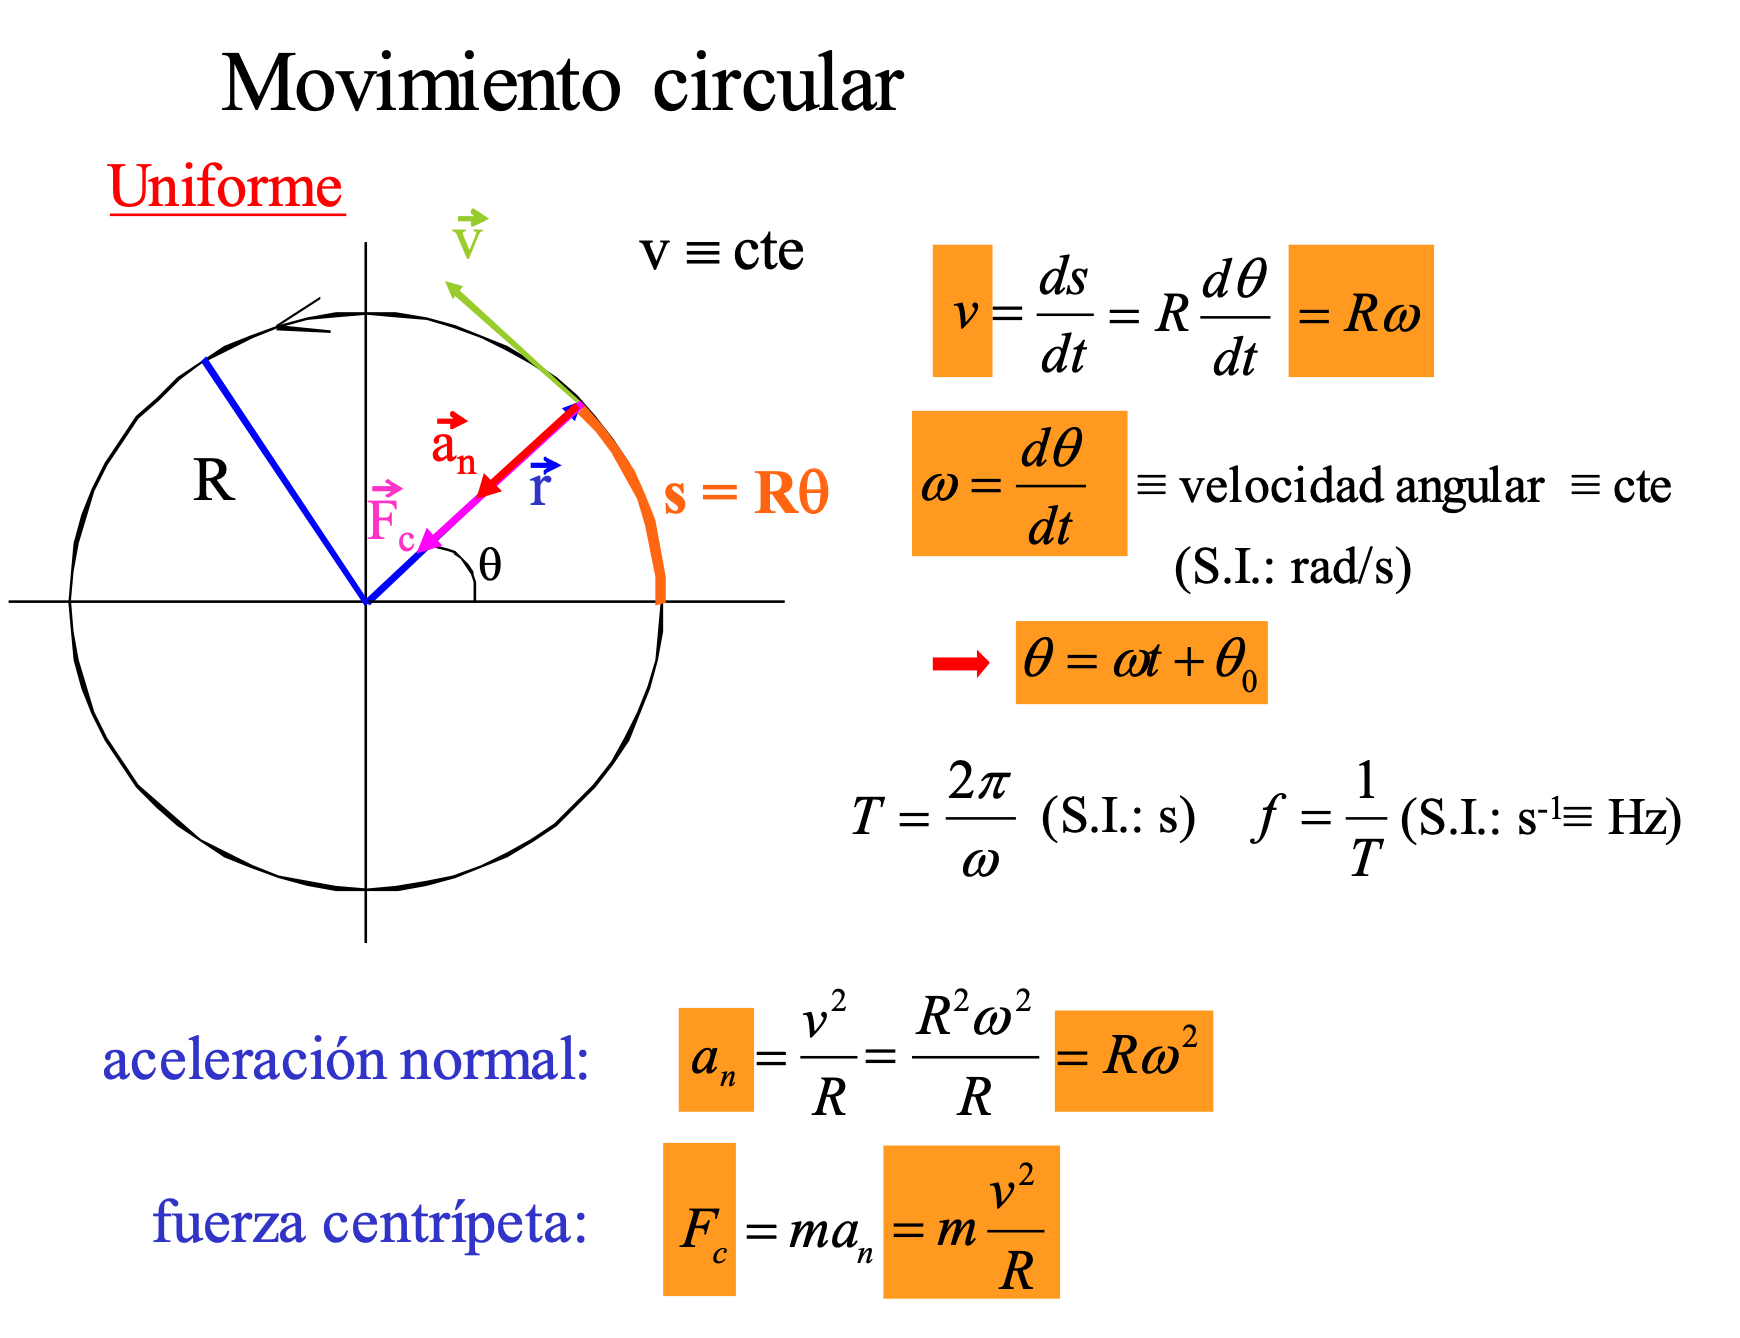
\includegraphics[width=.6\textwidth]{imagenes/imagenes02/T02IM31.png}
		\end{figure}
	\vspace{-5mm}\begin{figure}[H]
		\centering
		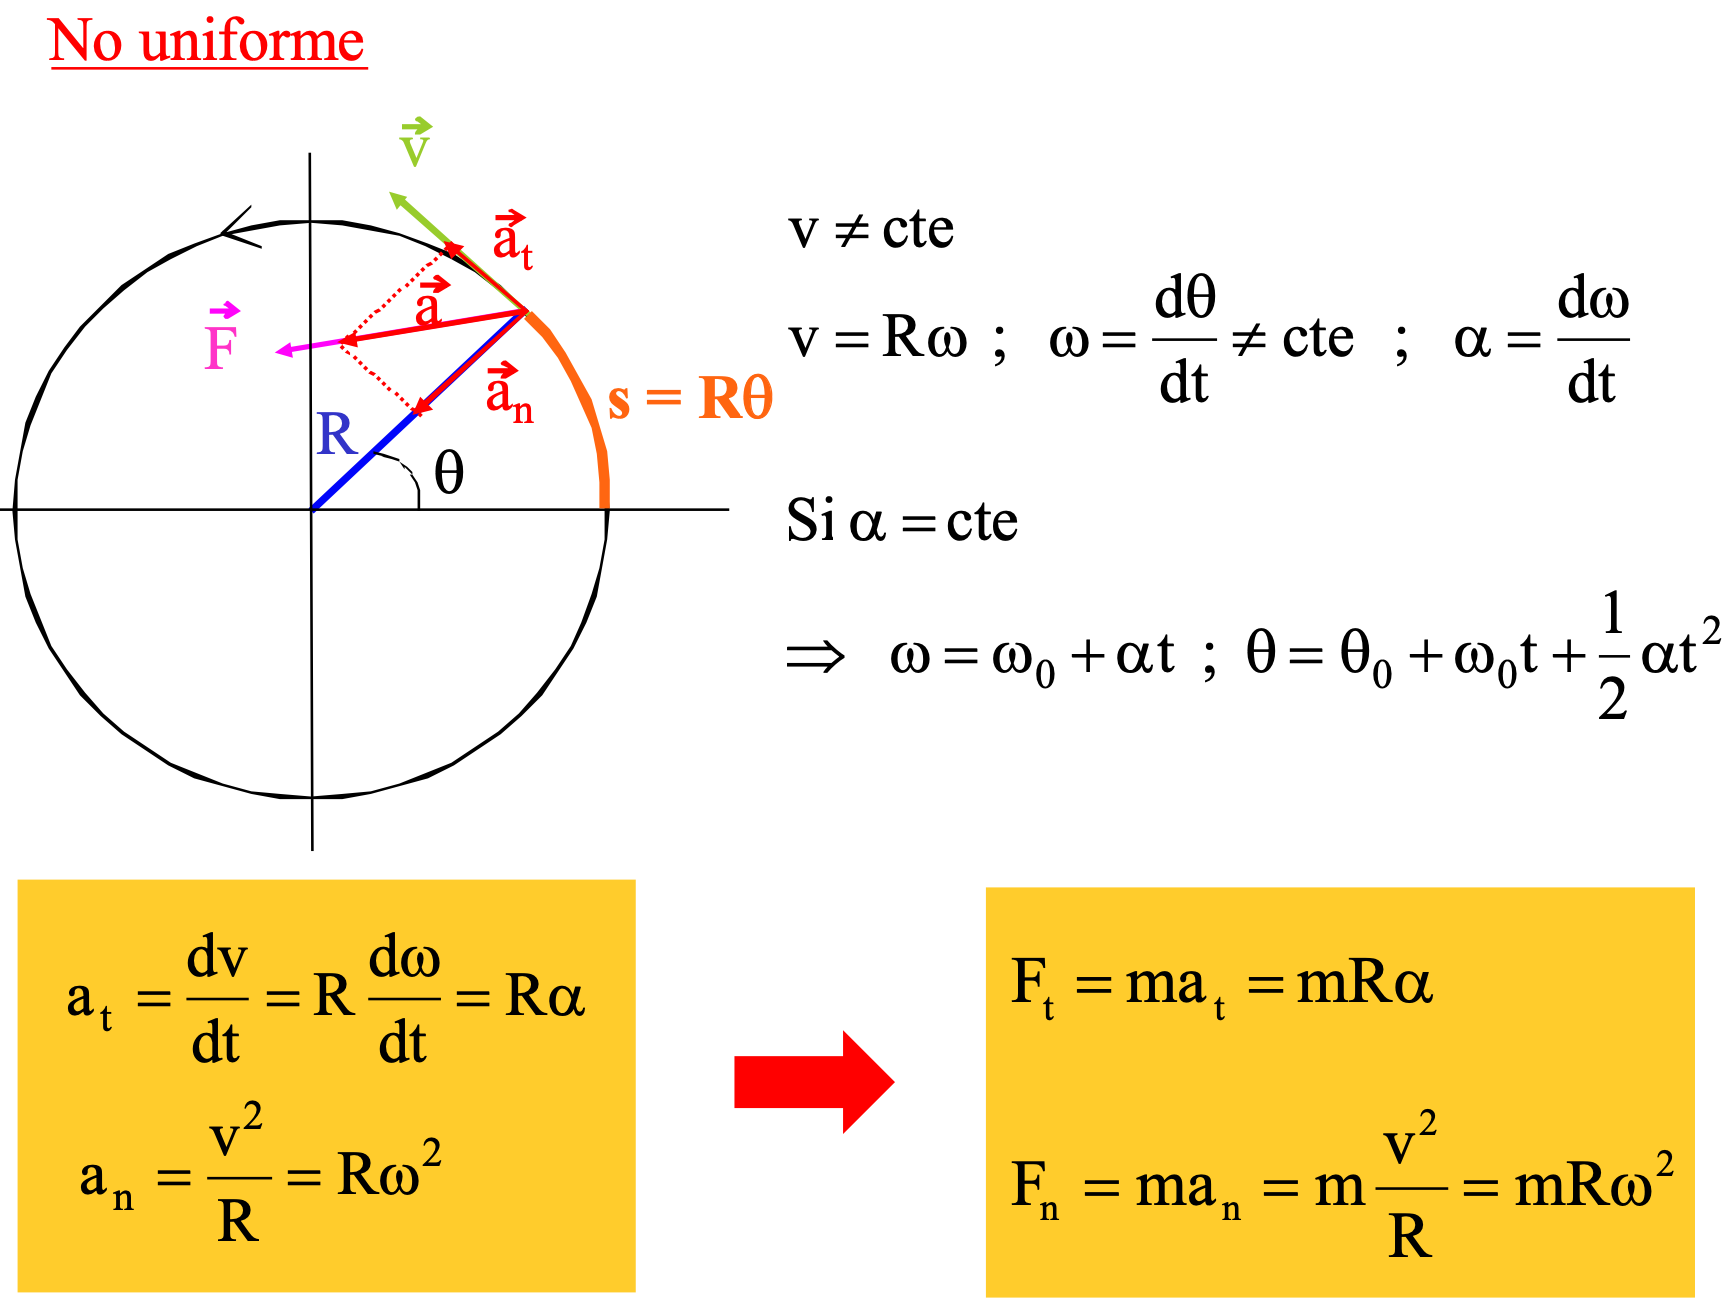
\includegraphics[width=.6\textwidth]{imagenes/imagenes02/T02IM32.png}
		\end{figure}


\section{Problemas}

\begin{prob}
Se está usando un vehículo robot para explorar la superficie de Marte. El módulo de descenso es el origen de coordenadas; en tanto que la superficie marciana circundante está en el plano $XY$. El vehículo, que representamos como un punto, tiene coordenadas x y y que varían con el tiempo según: $x=2-0.25t^2$, $y=t+0.025t^3$, estando $t$ en $\mathrm{s}$ y $x$ e $y$ en $\mathrm{m}$ 
\begin{quote}
\begin{enumerate}[a) ]
\item Obtenga las coordenadas del vehículo y su distancia con respecto al módulo en $t=2\;\mathrm{s}$ . 
\item Obtenga los vectores de desplazamiento y velocidad media del vehículo entre $t=2\;\mathrm{s}$ y $t=4\;\mathrm{s}$
\item Deduzca una expresión general para el vector de velocidad instantánea del vehículo. 
\item Exprese la velocidad instantánea en $t=2\; \mathrm{s}$ en forma de componentes y además en términos de magnitud y dirección.  
\item Obtenga el vector aceleración en cualquier instante $t$.
\item Obtenga las componentes de la aceleración en el instantes $t=2\; \mathrm{s}$. 
\item Obtenga las componentes paralela y perpendicular de la aceleración en $t = \;2 \mathrm{s}$. 
\end{enumerate}
\end{quote}	
\end{prob}
 $x=2-0.25t^2\qquad y=t+0.025t^3 \qquad t(\mathrm{s});\;\; x(\mathrm{m}),\; y(\mathrm{m})$
 
 --- a) $t=2\to x=1\;\mathrm{m};\quad y=8.2\; \mathrm{m}\; \quad \vec r=\vec i+8.2\vec j; \quad \abs{\vec r}=8.26\; \mathrm{m}$
 
 --- b) $\displaystyle \overline{\;\vec v\; }=\dfrac{\Delta \vec r}{\Delta t}=\dfrac{\vec r(4)-\vec r(2)}{4-2}$
 
$ \begin{cases}
 \vec r(4)=x(4)\; \vec i+ y(4)\vec j=-2 \vec i +9.6 \vec j
 \\
 \Delta r=(-2,9.6)-(1,8.2)=3\vec i+1.4\vec j 
\end{cases}
\displaystyle \overline{\;\vec v\; }=\dfrac {(3,1,4)}{4-2}=(\;1.5\vec i+0.7\vec j\;)\; \mathrm{ms}^{-1}$

$\abs{\displaystyle \overline{\;\vec v\; }}=\sqrt{1.5^2+0.7^2}=1.66\; \mathrm{ms}^{-1}$

--- c) $\vec v=\displaystyle\dv{\vec r}{t}= \dv{x}{t}\vec i+\dv{y}{t} \vec j= -0.5t\;\vec i + (1+0.075t^2)\;\vec j $

--- d) $t=2s \to \vec v(2)=-\vec i+1.3\; \vec j \to \abs{\vec v(2)}= 1.64\; \mathrm{ms}^{-1};\; \theta_{\vec v(2)}=\arctan \dfrac {v_y} {v_x}=127.6^o$, siendo $\theta_{\vec v(2)}$ el ángulo que forma el vector velocidad con semieje $OX+$ en el instante $t=2\; \mathrm{s}$.

--- e) $\displaystyle \vec a= \dv{\vec v}{t}=-0.5\;\vec i+ 0.15t\; \vec j$

--- f) $\vec a(2)=-0.5\;\vec i+0.3\vec j \quad \to \quad a_x=-0.5 \; ms^{-1}; \; \; a_y(2)=0.3\;\mathrm{ms}^{-2};$

$\displaystyle   \abs{\vec a(2)}= 0.58\; \mathrm{ms}^{-2};\quad \theta_{\vec a_2}=\arctan \dfrac {a_y} {a_x}=149.0^o$


--- g) A partir de los ángulos que forman los vectores $\vec v$ y $\vec a$ con el semieje $OX+$, $\theta_{\vec v}$ y $\theta_{\vec a}$ a los $t=2\; \mathrm{s}$, deducimos que el ángulo que forma el vector aceleración con la recta tangente a la trayectoria (dirección del vector velocidad) es $\theta=\theta_{\vec a(2)}-\theta_{\vec a(1)}=149.0-127.6=21.4^o$, en ese mismo instante, por lo que las componentes tangencial y normal de la aceleración son:




$a_T(2)=\abs{\vec a(2)}\; \cos \theta=0.54\; \mathrm{ms}^{-2}$
$;\quad$
$a_N(2)=\abs{\vec a(2)}\; \sin \theta=0.21\; \mathrm{ms}^{-2}$

\begin{figure}[H]
		\centering
		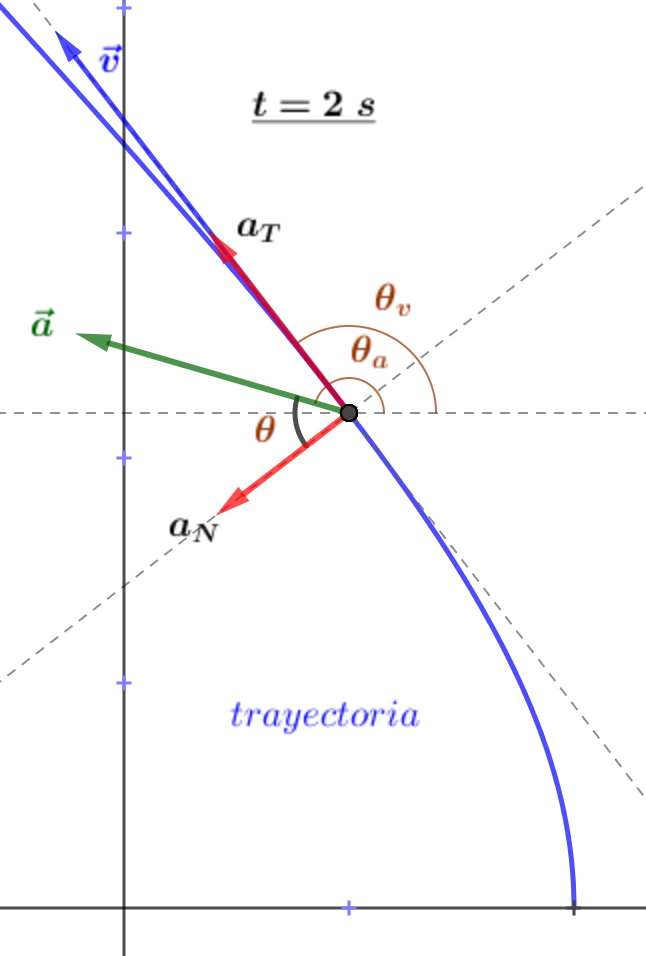
\includegraphics[width=.35\textwidth]{imagenes/imagenes02/T02IM19.png}
		\end{figure}


\begin{prob}
Una partícula se mueve en línea recta con una aceleración $a=-4v$, siendo $v$ su velocidad. Calcular la distancia que debe recorrer para que su velocidad se reduzca a $8\ \mathrm{ms}^{-1}$ y el tiempo necesario para ello si empezamos a contar cuando la velocidad de la partícula es de $80\ \mathrm{ms}^{-1}$.	
\end{prob}

$\displaystyle a=\dv{v}{t}=-4v \to \int_{v_0}^v \dfrac{\dd v}{v}=-\int_0^t 4 \dd t \to \ln \dfrac {v_0}{v}=4t \Rightarrow $ 

$\displaystyle t=\dfrac 1 4 \ln \dfrac {v_0}{v}=\dfrac 1 4 \ln \dfrac {80}{8}=0.58\ \mathrm{s}$

$\displaystyle a=\dv{v}{t}=\dv{v}{s}\ \dv{s}{t}=\dv{v}{s} \ v=-4v \to \dd v=-4 \ \dd s \to $

$\displaystyle \int_{v_0}^v
 \dd v=-4\int_0^s \dd s \to v-v_0=-4s \Rightarrow s=\dfrac 1 4 (v_0-v)=\dfrac 1 4 (80-8)=18\ \mathrm{m}$

\vspace{10mm} %********************************************
\begin{prob}
La velocidad angular de una rueda viene dada por la ecuación $\omega=2\ \theta^{1/2}$. Calcular el tiempo necesario para dar una vuelta completa así como la aceleración angular en cada instante. ?`Cómo es ese tipo de movimiento?	
\end{prob}
$\omega=\displaystyle \dv{\theta}{t}=2\ \theta^{1/2} \to \dd t=\dfrac{\dd \theta}{2\ \theta^{1/2}}=\dfrac{\dd \theta}{2\sqrt{\theta}}$

El tiempo en dar una vuelta completa, en barrer $2 \pi$ radianes, es el periodo T:

$\displaystyle T=\int_0^T \dd t=\int_0^{2 \pi} \dfrac{\dd \theta}{2\sqrt{\theta}}=\eval{\sqrt{\theta}}_0^{2 \pi}=\sqrt{2 \pi}$

Aceleración angular:

$\displaystyle \alpha= \dv{\omega}{t}=2 \frac 1 2 \theta^{-1/2} \dv{\theta}{t}=\theta^{-1/2} \ \omega =\theta^{-1/2}\ 2 \theta^{1/2}=2=cte.$ 

Como $\alpha=cte$, se trata de un MCUA (movimiento circular uniformemente acelerado).

\vspace{30mm} %********************************************

\begin{prob}
Calcúlese la velocidad angular de la tierra	
\end{prob}

\begin{multicols}{2}
Si utilizamos la relación \ref{periodo-vel-angular} $\;\omega=\dfrac {2\pi}T$ y consideramos $T=24\mathrm{h}=86400 \mathrm{s}$, cometemos un error debido al efecto que tiene la traslación de la tierra, pues al dar una vuelta completa en torno a su eje, el punto $P$ estaría en la posición $P'$ y deseamos que para definir el día vuelva a apuntar al sol, $P''$. Nos hemos pasado un ángulo $\gamma$. Como la traslación es de $365$ días aprox., $\gamma=360/365 =0.986^o\approx 0.017 \text{rad}$
\begin{figure}[H]
		\centering
		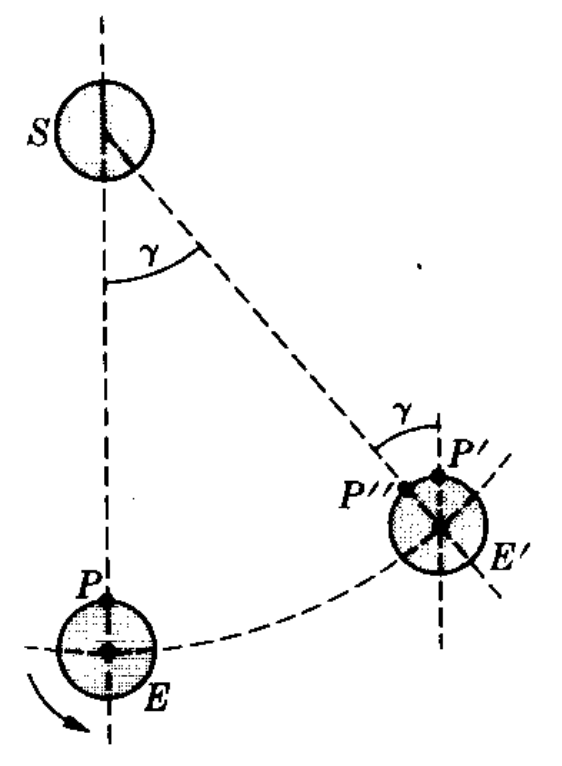
\includegraphics[width=.25\textwidth]{imagenes/imagenes02/T02IM18.png}
		\end{figure}
\end{multicols}

El tiempo $t$ aproximado para realizar ese giro por la rotación de la tierra sea corregido a  $t=\theta / \omega= 0.017 / (7.27\times 10^{-5}) \approx 234 \mathrm{s}$, donde hemos tomado como aproximación de $\omega_{rotac.}=2\pi / (24 \text{ días})=7.27\times 10^{-5}\; \mathrm{s}^{-1}$.

Esto hace que el periodo de rotación de la tierra sea $T=24horas - 234 s= 86400-234=86166\; \mathrm{s}$, con lo que:
$$\omega=\displaystyle \dfrac {2\pi}T=7.29\; \mathrm{s}^{-1}$$

\begin{prob}.

	\begin{multicols}{2}
La Tierra rota uniformemente respecto a su eje con una velocidad angular $\;\omega=7.3 \times 10^{-5}\;\mathrm{s}^{-1}\;$ (1 vuelta cada día). Encontrar, en función de la latitud, la velocidad y la aceleración de un punto situado en la superficie terrestre.
\begin{figure}[H]
		\centering
		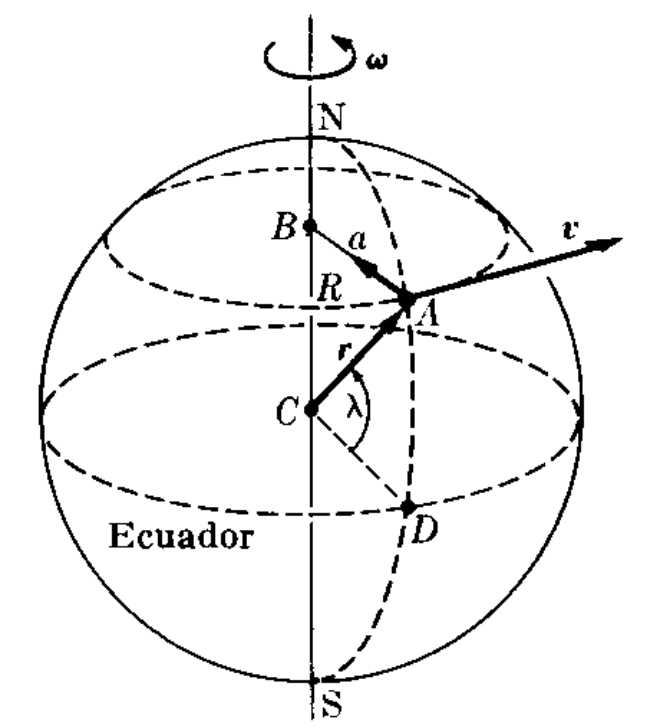
\includegraphics[width=.25\textwidth]{imagenes/imagenes02/T02IM17.png}
		\end{figure}
\end{multicols}
\end{prob}

Todos los puntos de la tierra se mueven con MRU, movimiento rectilíneo y uniforme ($\vec \omega =\overrightarrow{cte}$), luego $a_T=0$, solo hay $a_N$.

En la figura se observa que un punto A, situado a una latitud $\lambda$, describe una circunferencia paralela al ecuador de radio $r=R\; \cos \lambda$, con $R=\text{radio tierra}=6.4\times 10^6\; \mathrm{m}$.
El vector velocidad es tangente al paralelo $\lambda$, por tanto, paralelo al plano ecuatorial.

De  \ref{v-angular}: $\;\;\;v=\omega \cdot r =\omega\cdot R\cdot \cos \lambda$

De \ref{intrinsecas}: $\;\;a=a_N=\displaystyle \dfrac {v^2}r=\dfrac {\omega^2 \cdot r^2}r=\omega^2\cdot r=\omega\cdot R \cdot \cos \lambda$

Ambos valores máximos se alcanzan en el ecuador, $\lambda=0$:
$v_{max}(\lambda=0)=467 \;\mathrm{ms}^{-1}=1681.2\; \mathrm{kmh}^{-1};$

$ a=3.4\times 10^{-2} \; \mathrm{ms}^{-2} \sim 0.3\%\; g$

\vspace{10mm} %*************************************
\begin{prob}.
	\begin{figure}[H]
		\centering
		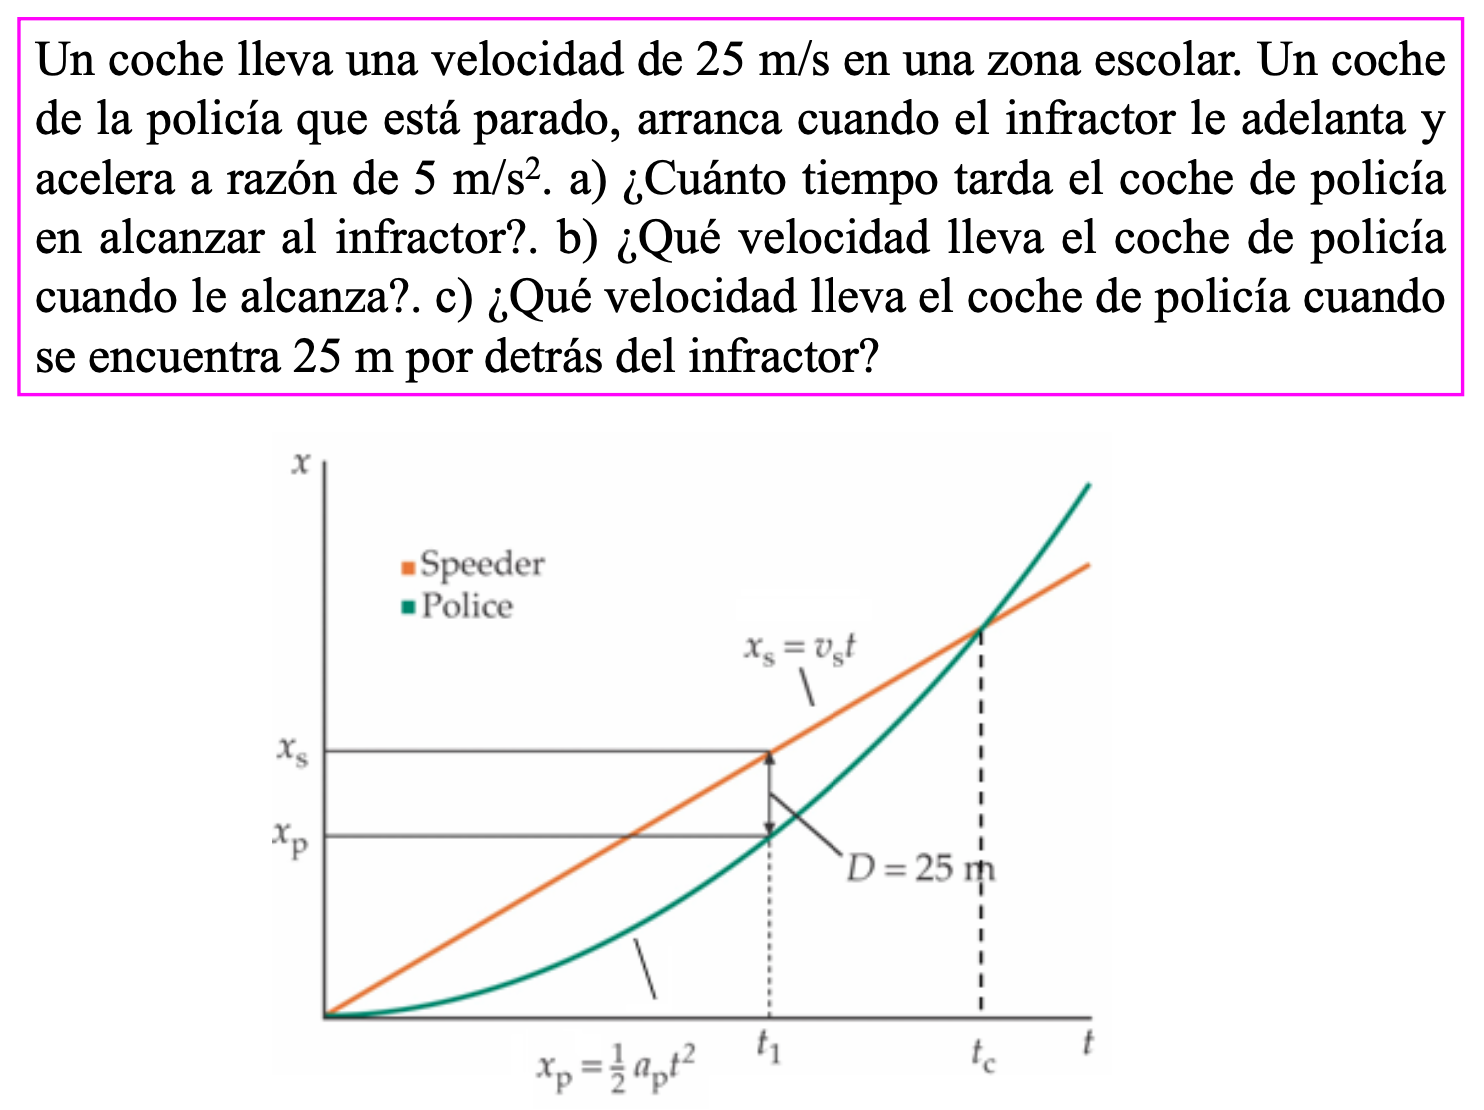
\includegraphics[width=.8\textwidth]{imagenes/imagenes02/T02IM25.png}
		\end{figure}
\end{prob}


\begin{prob}
Una esquiadora se mueve sobre una rampa de salto, como se muestra en la figura. La rampa es recta entre A y C, y es curva a partir de C. La rapidez de la esquiadora aumenta al moverse pendiente abajo de A a E, donde su rapidez es máxima, disminuyendo a partir de ahí. Dibuje la dirección del vector de aceleración en los puntos B, D, E y F	
\end{prob}
\begin{figure}[H]
		\centering
		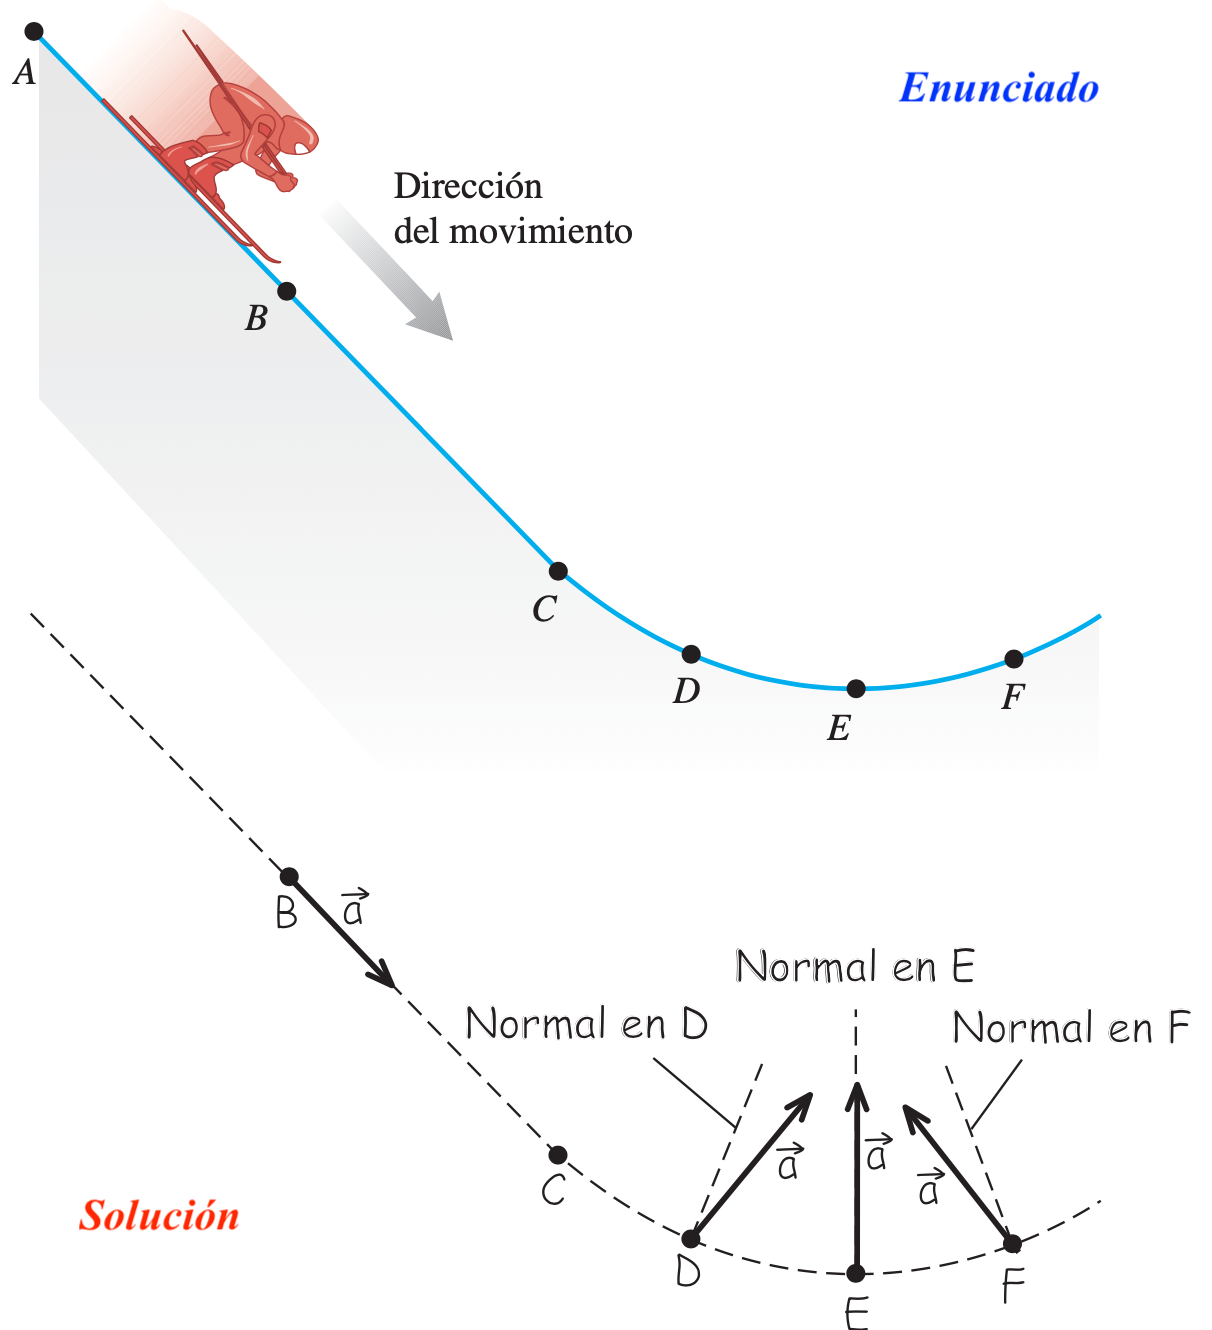
\includegraphics[width=.6\textwidth]{imagenes/imagenes02/T02IM16.png}
		\end{figure}

\vspace{30mm} %*************************************

\begin{prob}.
	\begin{figure}[H]
		\centering
		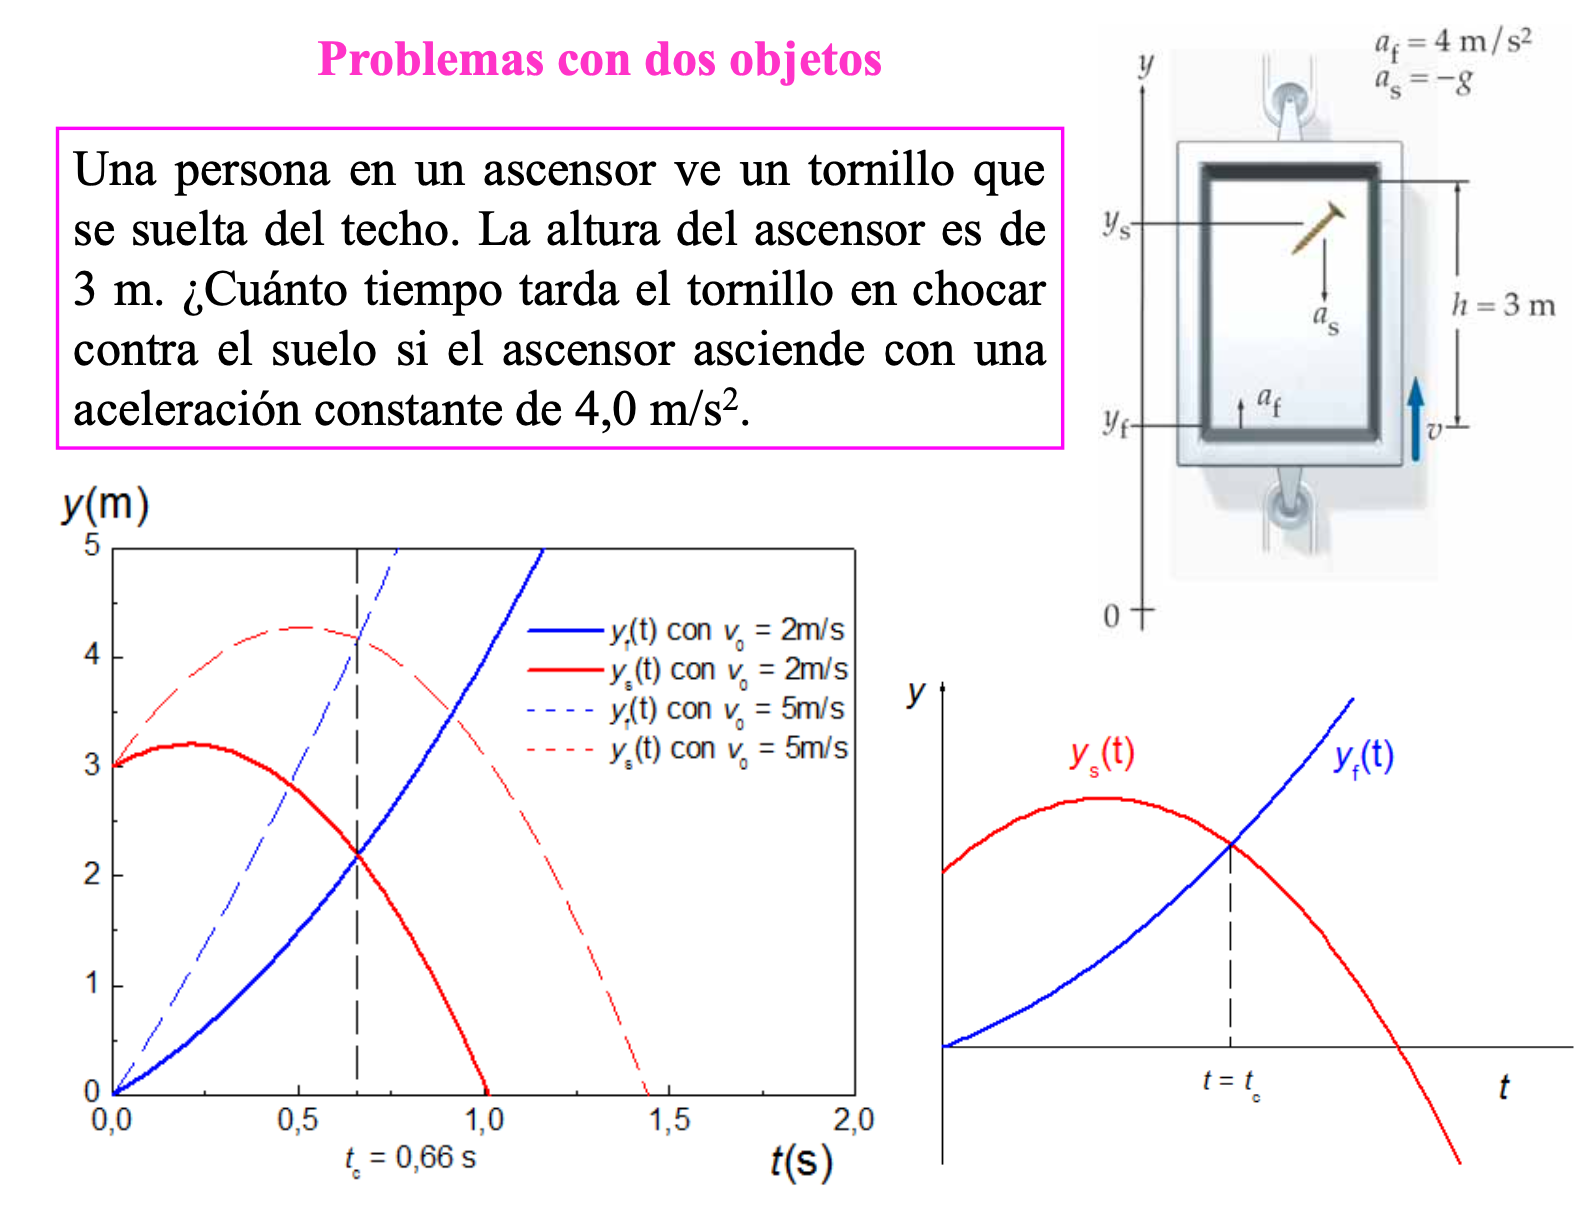
\includegraphics[width=.9\textwidth]{imagenes/imagenes02/T02IM26.png}
		\end{figure}
\end{prob}

\begin{prob}.
	\begin{figure}[H]
		\centering
		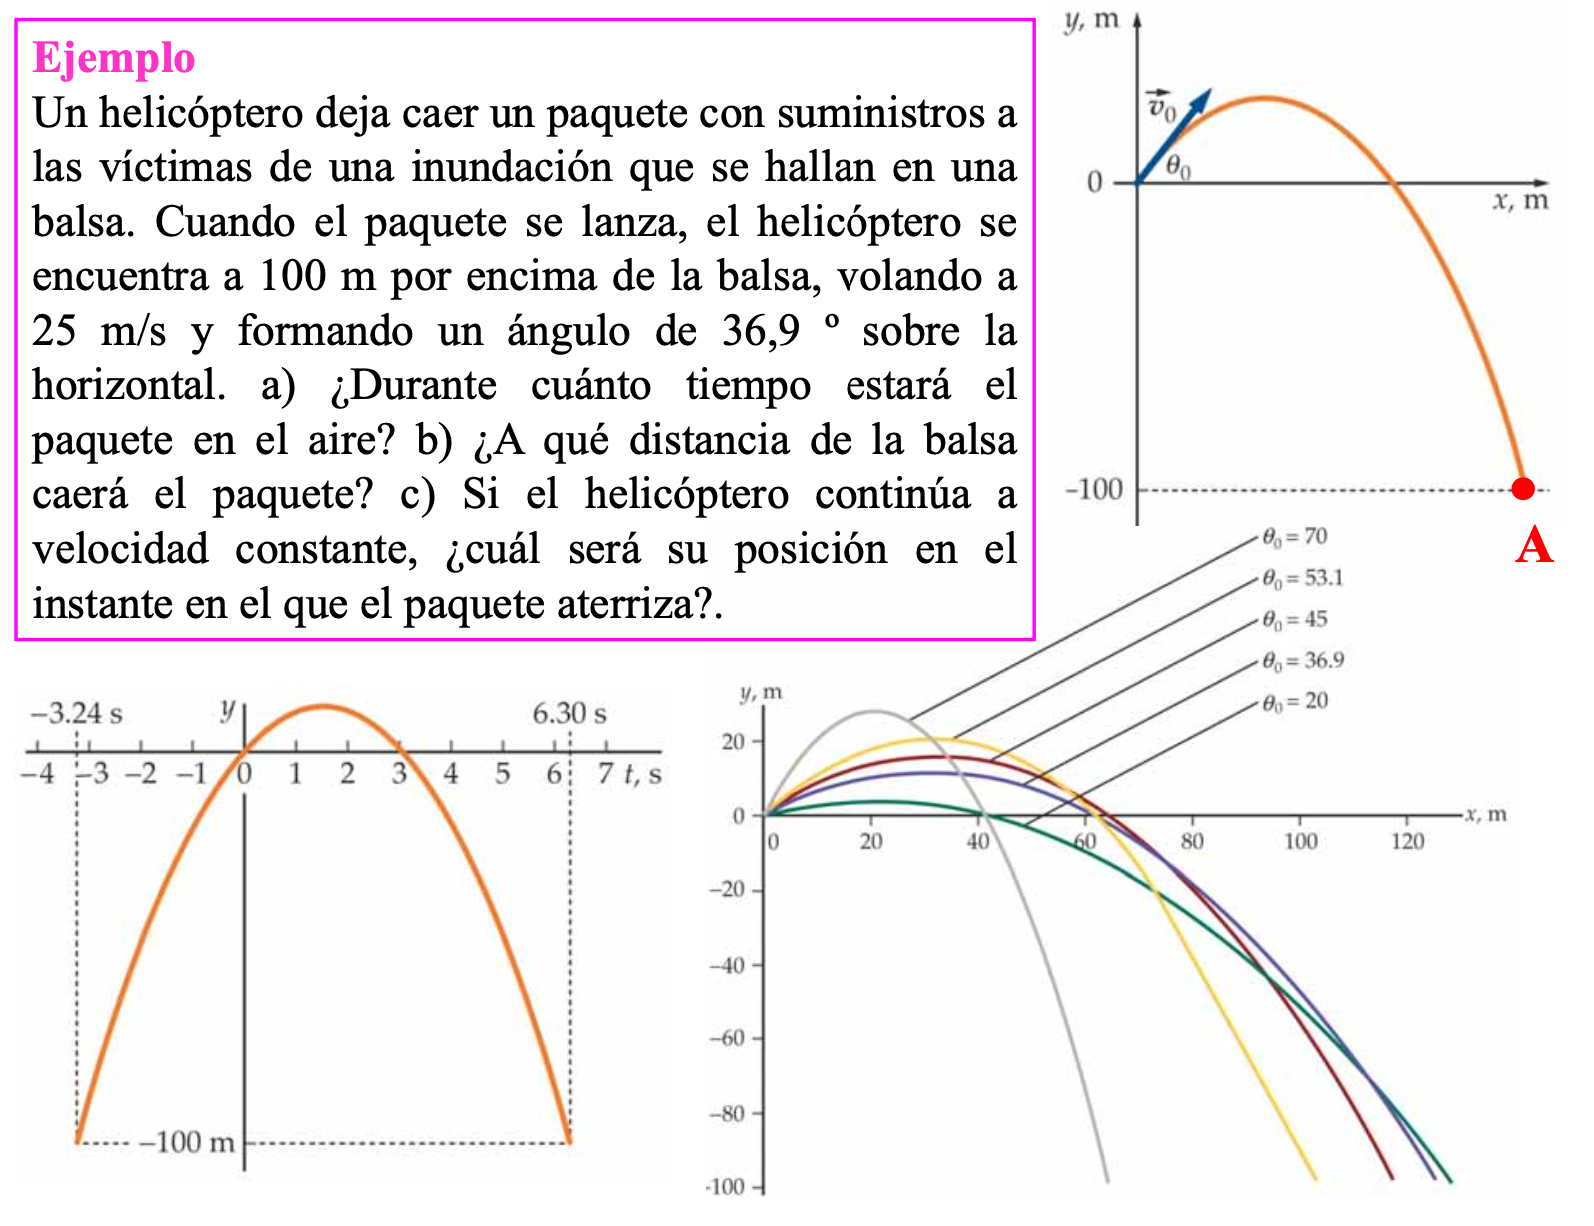
\includegraphics[width=.85\textwidth]{imagenes/imagenes02/T02IM27.png}
		\end{figure}
\end{prob}



\begin{prob} Tiro oblicuo.
\end{prob}	

\vspace{-5mm} \begin{figure}[H]
		\centering
		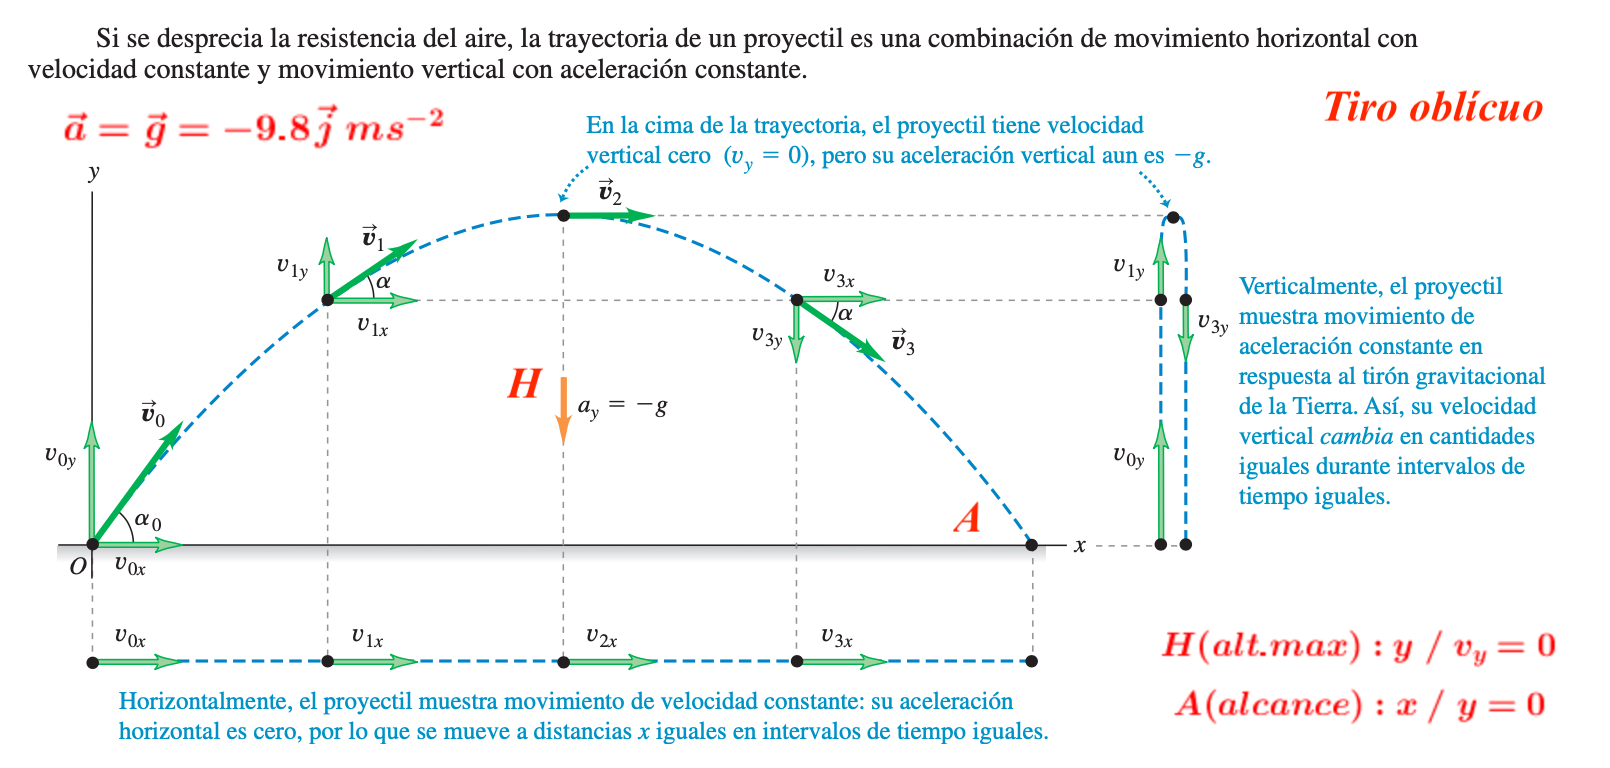
\includegraphics[width=1.1\textwidth]{imagenes/imagenes02/T02IM20.png}
		\end{figure}
		
\begin{prob} Un cazador dispara a un mono colgado de una rama. Demostrar que si el mono quiere vivir, no debe soltarse de la rama en el momento del disparo.
\end{prob}	
\begin{figure}[H]
		\centering
		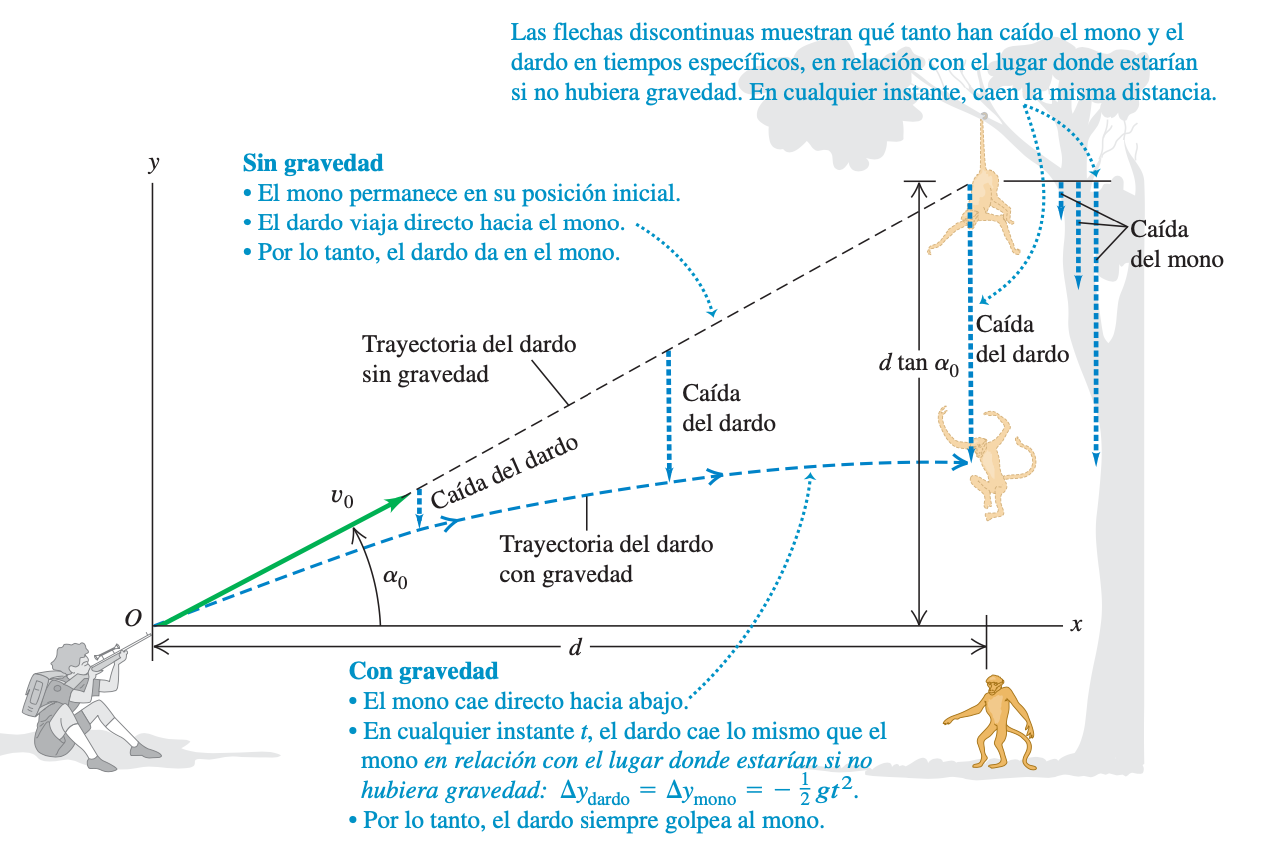
\includegraphics[width=1\textwidth]{imagenes/imagenes02/T02IM21.png}
		\end{figure}		





\begin{prob}
Una muchacha que está a $4\;\mathrm{m}$ de una pared vertical lanza contra ella una pelota que sale de su mano que está a $2 \; \mathrm{m}$ del suelo a una velocidad de $10\;\mathrm{ms}^{-1}$ y formando un ángulo de $45^o$ con la horizontal. Cuando la pelota choca contra la pared, se invierte la componente horizontal de la velocidad (rebote) mientras	 que su componente vertical continua sin variar. ¿Dónde caerá la pelota al suelo?

Comprobar que se puede considerar que la pared actúa como un espejo por lo que se puede resolver el problema como si no estuviese, calcular el alcance y, luego, considerar la reflexión especular de este punto respecto de la pared.
\end{prob}
\begin{figure}[H]
		\centering
		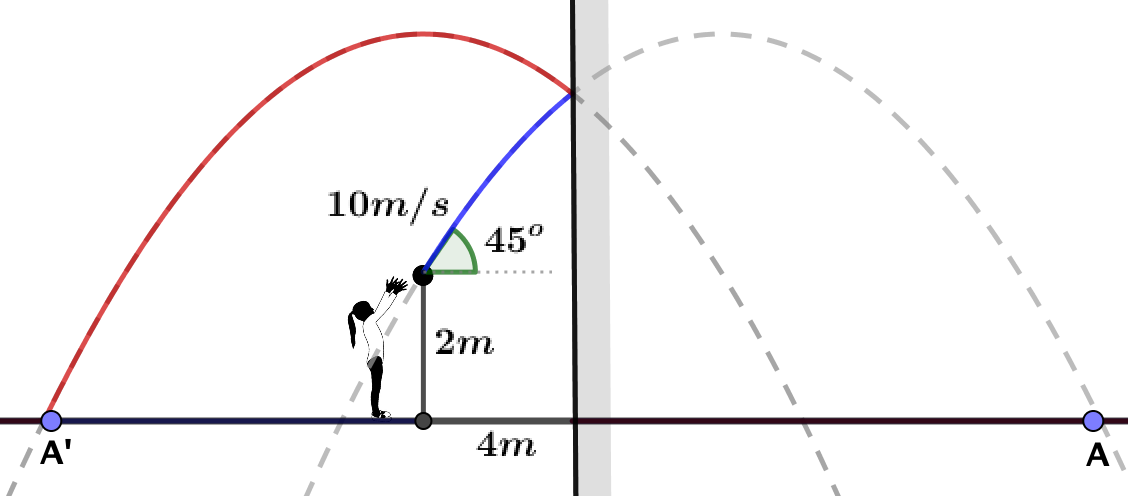
\includegraphics[width=.9\textwidth]{imagenes/imagenes02/T02IM24.png}
		\end{figure}
Dividimos el problema en dos: I- Desde el momento del tiro hasta que llega a la pared, y II- desde el rebote en la pared hasta que la pelota llega al suelo.

--- Parte I:  Colocamos el sistema de referencia en los pies de la niña u empezamos a contar el tiempo en el momento del lanzamiento, por tanto: $t_0=0\;\; x_0=0;\; y_0=2;\; v_{0_x}=v_x=v\cos \theta=10\cos 45^o=7.07;\; v_{0_y}=v\sin \theta=10\sin 45^o=7.07;\; a=g=-9.8\vec j\;$ Todo el el SI de unidades.

Cuando la pelota llega a la pared la distancia recorrida en el eje $X$ es de $4\;m$, el tiempo empleado es: $x=x_0+v_x\;t \to 4=0+7.07t \Rightarrow t=0.57\; \mathrm{s}$

Con el paso de este tiempo, calculamos la altura que ha alcanzado la pelota: $y=y_0+v_{0_y}\;t+\frac 1 2 \;a\;t^2 \to y=2+7.07\cdot 0.57-4.9\cdot 0.57^2 \Rightarrow y=4.44\; \mathrm{m}$

Calculemos, finalmente, la velocidad que lleva en su componente $y$ en ese momento: $v_y=v_{0_y}+a\; t \to v_y=7.07-9.8\cdot 0.57=1.48\; \mathrm{ms}^{-1}$

--- Parte II: Dejamos el sistema de referencia espacial a los pies de la niña pero vamos a cambiar, para facilitar el cálculo, el sistema de referencia temporal. Ahora empezamos a contar el tiempo en el momento del rebote en que se invierte el sentido de la componente $x$ del vector velocidad. Tendremos, pues: $t_0=0;\; x_0=4;\; y_0=4.44;\; v_{0_x}=v_x=-7.07;\; v_{0_y}=1.48;\; a=g=-9.8\vec j\;$, como antes, todo en el SI de unidades.

Calculemos el tiempo en que la pelota cae al suelo (desde el rebote). Eso ocurrirá cuando $y=0\to 0=4.44+1.48t-4.9t^2\Rightarrow t=1.11\; \mathrm{s}$.

Calculemos ahora la distancia recorrida durante ese tiempo por la pelota a lo largo del eje $x$: $\;x=4-7.07\cdot 1.11\approx -3.9\;\mathrm{m}$

CONCLUSIÓN: La pelota cae a $3.9\;\mathrm{m}$ a la izquierda de los pies de la niña.

\rule{150pt}{0.4pt} 

Resolvamos el problema suponiendo que la pared es un espejo. Inicialmente actuaremos como si no estuviese y, luego, calcularemos el punto simétrico del de impacto respecto de la pared-espejo.

De nuevo, colocamos el sistema de referencia en los pies de la niña u empezamos a contar el tiempo en el momento del lanzamiento, por tanto: $t_0=0\;\; x_0=0;\; y_0=2;\; v_{0_x}=v_x=v\cos \theta=10\cos 45^o=7.07;\; v_{0_y}=v\sin \theta=10\sin 45^o=7.07;\; a=g=-9.8\vec j\;$ Todo el el SI de unidades.

El tiempo de vuelo del proyectil lo encontraremos exigiendo que $y=0 \to y=y_0+v_{0_y}t+\frac 1 2 a t^2 \to 0=2+7.07t-4.9t^2 \Rightarrow t=1.69\;\mathrm{s}$

Con este tiempo, vamos a calcular el alcance de la pelota, la distancia recorrida en el eje $x$: $\; x=x_0+v_xt\to x=0+7.07\cdot 1.69=11.9\;\mathrm{m}$

Es decir, si no hay pared-espejo, la pelota cea a $11.9\;\mathrm{m}$ de los pies de la niña, es decir, a $11.9-4=7.9\;\mathrm{m}$ de la pared.  El simétrico de $+7.9\;\mathrm{m}$ de la pared es $-7,9\;\mathrm{m}$ de la misma, es decir, a su izquierda. Como la niña está a $4\:\mathrm{m}$ a la izquierda de la pared, la pelota caerá, pues, a $7.9-4=3.9\;\mathrm{m}$ a la izquierda de la niña.

\begin{prob}
Conduces un automóvil por una autopista recta. En el instante $t = 0$, cuando avanzas a $10 \ \mathrm{ms}^{-1}$ en la dirección $+x$, pasas un letrero que está en $x= 50 \ \mathrm{m}$. Tu aceleración es una función del tiempo: $_x = (2.0 - 0.10 t)\ \mathrm{ms}^{-2}$. 

a) Deduce las expresiones para tu velocidad y posición en función del tiempo.  

b) ¿En qué momento es máxima tu velocidad?  

c) ¿Cuál es esa velocidad máxima?  
\end{prob}
$v=10+2t-0.05t^2$ 

$x=50+10t+t^2-0.017t^3$

$a=0$ si $t=20 \to v_{max}=30\ \mathrm{ms}^{-1}$	

\begin{prob}
Sabemos demostrar que, en ausencia de rozamiento con el aire, el alcance máximo de un cuerpo que sigue un movimiento parabólico se consigue para un lanzamiento a $45^o$ sobre la horizontal (siempre que el punto de lanzamiento y el de impacto se encuentren a la misma altura). ¿Es también cierto cuando el suelo está inclinado? 
\end{prob}
\begin{multicols}{2}
Datos: $\vec v_0,\;\; \theta,\;\; \phi$

A encontar $d=d(\vec v_0,\theta,\phi)$

Para $v_0, \ \theta \ { y }\  \phi$ dados $\to d_{max}(\phi)$
\begin{figure}[H]
		\centering
		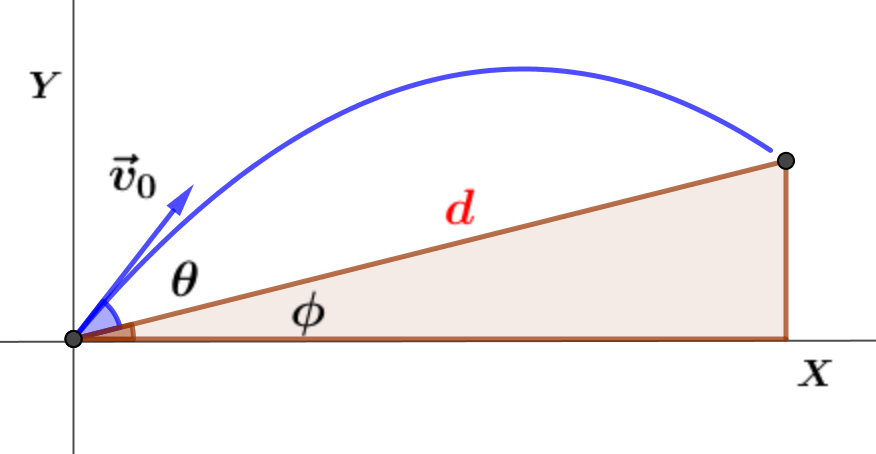
\includegraphics[width=.5\textwidth]{imagenes/imagenes02/T02IM36.png}
		\end{figure}
\end{multicols}

Sistema de referencia en punto de lanzamiento y empezamos a contar el tiempo en el momento del mismo: $x_0=y_0=t=0$.

Buscamos la ecuación de la trayectoria parabólica que describe el proyectil. Partimos de las ecuaciones de las posiciones:

$\begin{cases} x=v_0 \cos (\theta+\phi) \ t \\ y=v_0 \sin (\theta+\phi) \ t - \frac g 2 t^2 \end{cases}  \to t=\dfrac x{v_0 \cos (\theta+\phi)} $

$\Rightarrow y=\cancel{v_0} \sin (\theta+\phi) \dfrac x{\cancel{v_0} \cos (\theta+\phi)} - \dfrac g 2 \left( \dfrac x{v_0 \cos (\theta+\phi)}  \right)^2$

La ecuación de la trayectoria (parábola) es:

$\textcolor{blue}{y=\tan(\theta+\phi) \ x - \dfrac {g}{2 v_0^2 \cos^2 (\theta+\phi)}\ x^2}$

Por otra parte, la ecuación del plano inclinado es:

$\textcolor{red}{y}=mx\textcolor{red}{=\tan \phi \ x}$

El punto de impacto del \textcolor{blue}{proyectil} contra el \textcolor{red}{suelo} se producirá en la \textbf{intersección} de la \textcolor{blue}{parábola (trayectoria)} con la \textcolor{red}{recta (plano inclinado)}. Igualando ambas expresiones:

$\tan(\theta+\phi) \ x - \dfrac {g}{2 v_0^2 \cos^2 (\theta+\phi)}\ x^2=\tan \phi \ x$

$x\cdot \left[ 
\tan(\theta+\phi) \ x - \dfrac {g}{2 v_0^2 \cos^2 (\theta+\phi)}\ x^2=\tan \phi \ x
 \right]=0 \to  \begin{cases} x=0 \,(inicio) \\ [ \; ]=0 \to \end{cases}$


$[\;]\to x=\left[\tan (\theta+\phi)-\tan \phi  \right] \  \dfrac{2v_0^2 \cos^2(\theta+\phi)}{g} =$

$=\dfrac {\sin(\theta+\phi) \cos \phi-\sin \phi \cos(\theta+\phi)}{\cos(\theta+\phi) \cos \phi} \  \dfrac{2v_0^2 \cos^2(\theta+\phi)}{g} =$

$=\dfrac {\sin [(\theta+\phi)-\phi]}{\cos(\theta+\phi) \cos \phi} \ \dfrac{2v_0^2 \cos^2(\theta+\phi)}{g} $
$=\dfrac {\sin \theta}{\cancel{\cos(\theta+\phi)} \cos \phi} \ \dfrac{2v_0^2 \cos^{\cancel{2}}(\theta+\phi)}{g} =$


Luego, las coordenadas del punto de impacto son:

$x=\dfrac{2v_0^2}{g}\ \dfrac {\sin \theta \ \cos (\theta+\phi)}{\cos \phi}; \qquad y\ \textcolor{gris}{=\tan \phi \ x }= \tan \phi \ \dfrac{2v_0^2}{g}\ \dfrac {\sin \theta \ \cos (\theta+\phi)}{\cos \phi}$

La longitud $d$ del plano inclinado a que el proyectil impacta sobre el plano inclinado, la podemos calcular por trigonometría:

$\cos \phi = \dfrac x d \to \quad \boldsymbol{d= \dfrac{2v_0^2}{g}\ \dfrac {\sin \theta \ \cos (\theta+\phi)}{\cos^2 \phi} }$ 


Para encontrar el ángulo de tiro $\theta$ que para una velocidad inicial dada $v_0=cte$ y una inclinación del plano dada $\phi=cte$, lo obtendremos sin más que derivar $d=d(\theta)$, con $v_0$ y $\phi$ constantes. 

$d'=\dfrac {2 v_0^2}{g  \cos^2 \phi}\ \left[ \cos \theta \cos (\theta+\phi) - \sin \theta \sin(\theta+\phi) \right]=0 \to $

$ \to \quad \tan (\theta + \phi)=\cot \theta \to \dfrac {\tan \theta + \tan \phi}{1-\tan\theta \tan \phi}=\dfrac {1}{\tan \theta} \to $

$\tan^2 \theta +2\tan\phi \tan \theta -1 =0 \Rightarrow \tan \theta= \dfrac {-2\tan \phi \pm \sqrt{4\tan^4 \phi+4}}{2}=-\tan \phi \pm \sqrt{\tan^2 \phi + 1}=-\tan \phi + \dfrac{1}{\cos \phi} \to \quad \boldsymbol { \tan \theta = \dfrac {1-\sin \phi}{\cos \phi} }$


Llevemos estos resultado a la ecuación que da $d$ para obtener el $d_{max}$

como $\cos \theta \textcolor{gris}{= \dfrac 1 {\sqrt{\tan^2}}} =\dfrac {\cos \phi}{\sqrt{2} \sqrt{1-\sin \phi}}; \qquad \sin \theta \textcolor{gris}{=\cos \theta \tan \theta}=\dfrac{\sqrt{1-\sin \phi}}{\sqrt{2}}$

$ d_{max}  =\dfrac {2 v_0^2}{g \cos^2 \phi} \dfrac {\sqrt{1-\sin \phi}}{\sqrt{2}} \left[
\dfrac {\cos \phi}{\sqrt{2}\sqrt{1-\sin \phi}}\cos \phi - \dfrac{\sqrt{1-\sin \phi}}{\sqrt{2}}\sin \phi
\right] $ 

$\boldsymbol{d_{max}} =\dfrac{\cancel{2} v_0^2}{g \cos^2 \phi \ \cancel{2}}[ \ \cos^2 \phi - (1-\sin \phi)\ \sin \phi  \ ]  = \boldsymbol{\dfrac {v_0^2 \ (1-\sin \phi)}{g \ \cos^2 \phi}}$

\vspace{4mm} \textbf{Análisis de dimensiones:} Las razones trigonométricas carecen de dimensiones. $[d]=\dfrac{[(LT^{-1})^2]}{[LT^-{-2}]}=[L]$

\vspace{4mm} \textbf{Análisis de casos extremos:}
\begin{itemize}
\item $\phi=0 \to d=\dfrac {v_0^2} {g}$, que coincide con lo previsto en tiro horizontal para $\theta=45^o$
\item$\phi=90^o \to d= \dfrac {v_0^2}{g}\ \eval{\dfrac {1-\sin \phi}{\cos^2 \phi}}_{\phi\to \pi/2}= [ \widetilde{\phi} =\pi/2 - \phi]=$ 

$= \dfrac {v_0^2}{g}\ \eval{\dfrac {1-\cos \widetilde{\phi}}{\sin^2 \widetilde{\phi}}}_{\widetilde{\phi}\to 0}=[McLauirin]= \dfrac {v_0^2} {g} \eval{\ \dfrac {1-\left( 1-\dfrac {1}{\widetilde{\phi^2}} \right)} {\widetilde{\phi^2}}}_{\widetilde{\phi}\to 0} =\dfrac {v_0^2}{2g}$, que coincide con la altura máxima alcanzada por un proyectil en tiro vertical.
\end{itemize}

\begin{prob}
Un esquiador deja una rampa de salto con una velocidad d $10 \ \mathrm{ms}^{-1}$	formando un ángulo de $15^o$ con la horizontal. La inclinación de la pista de salto es de $50^o$ y la resistencia del aire se considera despreciable. Encuéntrese la distancia $d$ a la que cae el esquiador a lo largo de la pista.
\end{prob}

\begin{multicols}{2}

\begin{figure}[H]
		\centering
		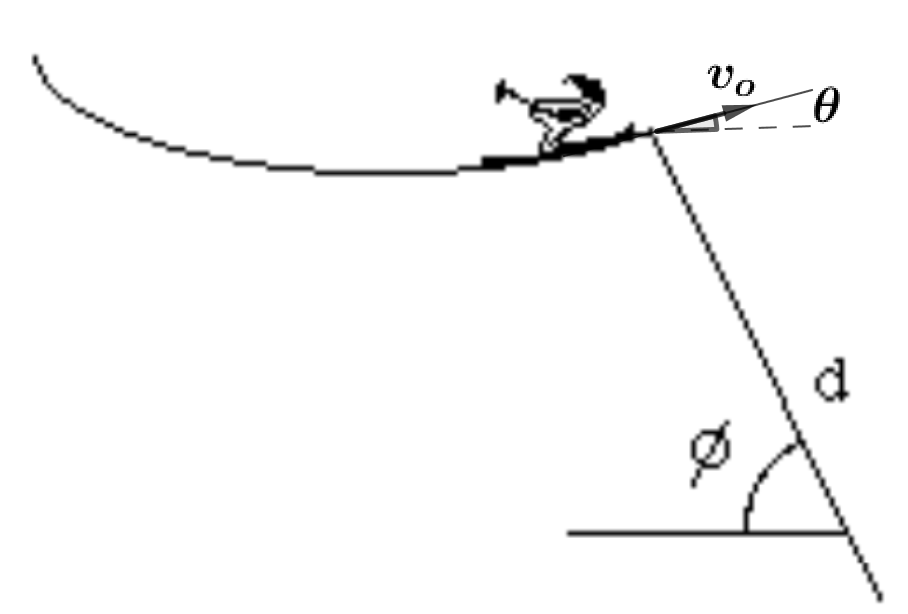
\includegraphics[width=.5\textwidth]{imagenes/imagenes02/T02IM37.png}
		\end{figure}
El problema es similar al anterior pero para $\phi>90^o$. 
Llamando al ángulo del plano inclinado $-\phi$, podremos usar las fórmulas anteriores.

\begin{figure}[H]
		\centering
		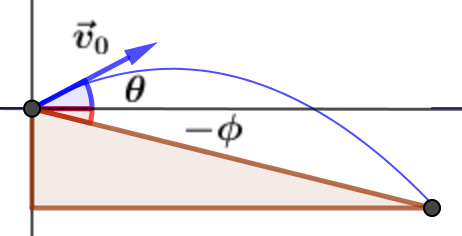
\includegraphics[width=.3\textwidth]{imagenes/imagenes02/T02IM38.png}
		\end{figure}

\end{multicols}


\vspace{-3mm}\begin{figure}[H]
		\centering
		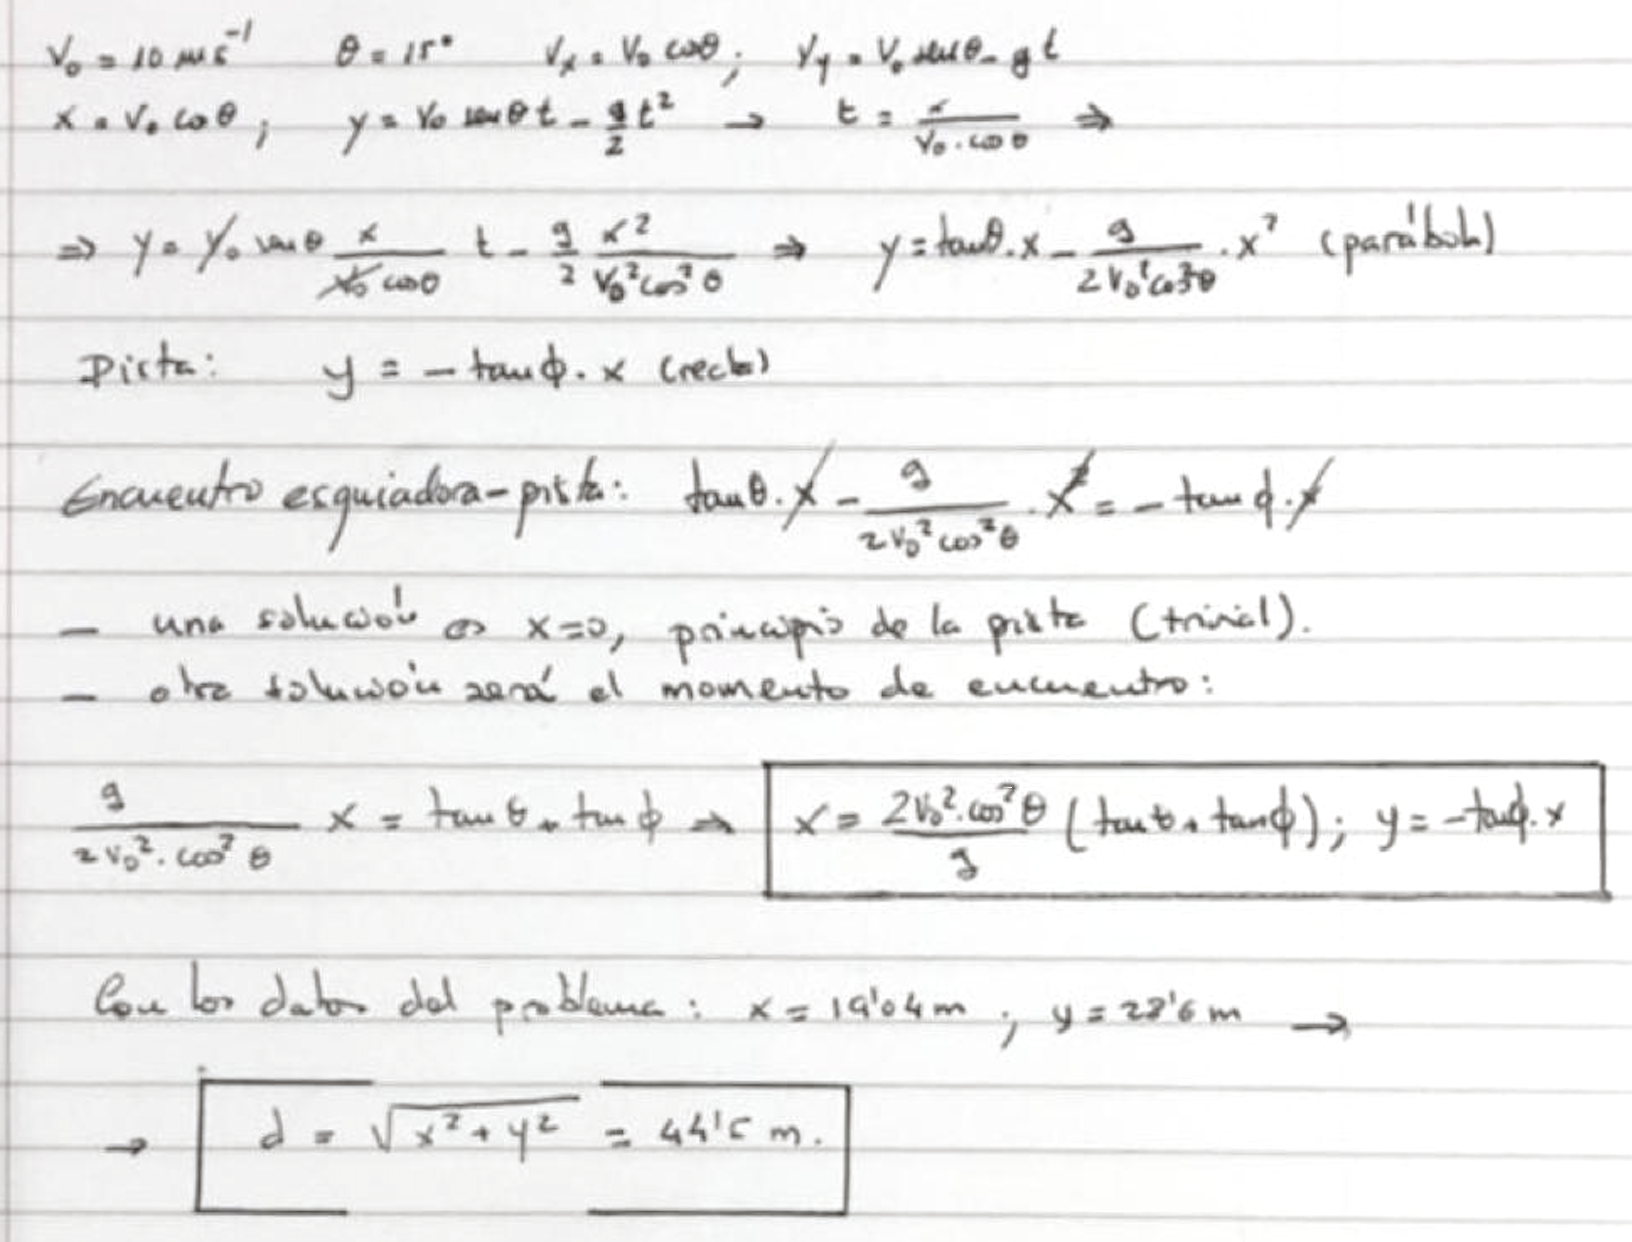
\includegraphics[width=1\textwidth]{imagenes/imagenes02/T02IM40.png}
		\end{figure}
		
	
		
\vspace{-3mm}\textbf{Análisis de casos límites:} 

Si en la expresión encontrada, $x=\dfrac{2v_0 \cos^2 \theta}{g}(\tan \theta+\tan \phi)$, hacemos $\phi=0$, se obtiene $x=\dfrac{v_0^2}{g} \sin 2\theta=x_{max}$, alcance máximo de un proyectil en superficie horizontal.

\newpage %**************************************

\begin{myblock}{Cinemática}
	
\begin{small}
El nacimiento de la cinemática moderna tiene lugar con la alocución de Pierre Varignon el 20 de enero de 1700, ante la Academia Real de las Ciencias de París. Fue allí cuando definió la noción de aceleración y mostró cómo es posible deducirla de la velocidad instantánea utilizando un simple procedimiento de cálculo diferencial.

\vspace{2mm} En la segunda mitad del siglo XVIII se produjeron más contribuciones por Jean Le Rond d'Alembert, Leonhard Euler y André-Marie Ampère y continuaron con el enunciado de la ley fundamental del centro instantáneo de rotación en el movimiento plano, de Daniel Bernoulli.

\vspace{2mm} El vocablo cinemática fue creado por André-Marie Ampère, quien delimitó el contenido de esta disciplina y aclaró su posición dentro del campo de la mecánica. Desde entonces, la cinemática ha continuado su desarrollo hasta adquirir una estructura propia.

\vspace{2mm} Con la teoría de la relatividad especial de Albert Einstein en 1905, se inició una nueva etapa, la cinemática relativista, donde el tiempo y el espacio no son absolutos, y sí lo es la velocidad de la luz.

\vspace{2mm} Los elementos básicos de la cinemática son el espacio, el tiempo y un móvil.

\vspace{2mm} La cinemática trata del estudio del movimiento de los cuerpos en general y, en particular, el caso simplificado del movimiento de un punto material, mas no estudia por qué se mueven los cuerpos sino que se limita a describir sus trayectorias y modo de reorientarse en su avance.

\vspace{2mm} El movimiento trazado por una partícula lo mide un observador respecto a un sistema de referencia. Desde el punto de vista matemático, la cinemática expresa cómo varían las coordenadas de posición de la partícula (o partículas) en función del tiempo. La función matemática que describe la trayectoria recorrida por el cuerpo (o partícula) depende de la velocidad (la rapidez con la que cambia de posición un móvil) y de la aceleración (variación de la velocidad respecto del tiempo).

\vspace{2mm} \textbf{Tipos de movimientos}:

--- Si la aceleración es nula, da lugar a un movimiento rectilíneo uniforme y la velocidad permanece constante a lo largo del tiempo.

--- Si la aceleración es constante con igual dirección que la velocidad, da lugar al movimiento rectilíneo uniformemente acelerado y la velocidad variará a lo largo del tiempo.

--- Si la aceleración es constante con dirección perpendicular a la velocidad, da lugar al movimiento circular uniforme, donde el módulo de la velocidad es constante, cambiando su dirección con el tiempo.

--- Cuando la aceleración es constante y está en el mismo plano que la velocidad y la trayectoria, tiene lugar el movimiento parabólico, donde la componente de la velocidad en la dirección de la aceleración se comporta como un movimiento rectilíneo uniformemente acelerado, y la componente perpendicular se comporta como un movimiento rectilíneo uniforme, y se genera una trayectoria parabólica al componer ambas.

--- Cuando la aceleración es constante pero no está en el mismo plano que la velocidad y la trayectoria, se observa el efecto de Coriolis.

--- En el movimiento armónico simple se tiene un movimiento periódico de vaivén, como el del péndulo, en el cual un cuerpo oscila a un lado y a otro desde la posición de equilibrio en una dirección determinada y en intervalos iguales de tiempo. La aceleración y la velocidad son funciones, en este caso, sinusoidales del tiempo.


\vspace{2mm} Un movimiento interesante es el de una peonza, que al girar puede tener un movimiento de precesión y de nutación. Cuando un cuerpo posee varios movimientos simultáneamente, como por ejemplo uno de traslación y otro de rotación, se puede estudiar cada uno por separado en el sistema de referencia que sea apropiado para cada uno, y luego, superponer los movimientos.

\vspace{2mm} \textbf{Movimiento sobre la Tierra}:

\vspace{2mm} Supongamos que un cañón situado en el ecuador lanza un proyectil hacia el norte a lo largo de un meridiano. Un observador situado al norte sobre el meridiano observa que el proyectil cae al este de lo predicho, desviándose a la derecha de la trayectoria. De forma análoga, si el proyectil se hubiera disparado a lo largo del meridiano hacia el sur, el proyectil también se habría desviado hacia el este, en este caso hacia la izquierda de la trayectoria seguida. La explicación de esta «desviación», provocada por el Efecto Coriolis, es debida a la rotación de la Tierra. El proyectil tiene una velocidad con tres componentes: las dos que afectan al tiro parabólico, hacia el norte (o el sur) y hacia arriba, respectivamente, más una tercera componente perpendicular a las anteriores debida a que el proyectil, antes de salir del cañón, tiene una velocidad igual a la velocidad de rotación de la Tierra en el ecuador. Esta última componente de velocidad es la causante de la desviación observada pues si bien la velocidad angular de rotación de la Tierra es constante sobre toda su superficie, no lo es la velocidad lineal de rotación, la cual es máxima en el ecuador y nula en el centro de los polos. Así, el proyectil conforme avanza hacia el norte (o el sur), se mueve más rápido hacia el este que la superficie de la Tierra, por lo que se observa la desviación mencionada. Lógicamente, si la Tierra no estuviese rotando sobre sí misma, no se daría esta desviación.

\vspace{2mm} Otro caso interesante de movimiento sobre la Tierra es el del péndulo de Foucault. El plano de oscilación del péndulo no permanece fijo, sino que lo observamos girar, girando en sentido horario en el hemisferio norte y en sentido antihorario en el hemisferio sur. Si el péndulo se pone a oscilar en el ecuador, el plano de oscilación no cambia. En cambio, en los polos, el giro del plano de oscilación toma un día. Para latitudes intermedias toma valores mayores, dependiendo de la latitud. La explicación de tal giro se basa en los mismos principios hechos anteriormente para el proyectil de artillería \end{small}\normalsize{.}
\end{myblock}



